\documentclass[]{scrartcl}

%%% PACKAGES
\usepackage[english]{babel}
%\usepackage[T1]{fontenc} % pouzije EC fonty
\usepackage[utf8]{inputenc} % set input encoding (not needed with XeLaTeX) 
\usepackage{lmodern}
\usepackage{graphicx} % support the \includegraphics command and options

\usepackage{caption}

\usepackage{subfig}
\usepackage{cite}
\usepackage{url}
\usepackage{epstopdf}
\usepackage{float}

\usepackage{amsmath}

% poziti pro vypis kodu
\usepackage{listings}
\usepackage{xcolor}

\definecolor{mygreen}{rgb}{0,0.6,0}
\definecolor{mygray}{rgb}{0.5,0.5,0.5}
\definecolor{mymauve}{rgb}{0.58,0,0.82}
% sets appearance of listings
\lstset{ %
	backgroundcolor=\color{yellow!20},   % choose the background color; you must add \usepackage{color} or \usepackage{xcolor}
	basicstyle=\scriptsize,        % the size of the fonts that are used for the code
	breakatwhitespace=false,         % sets if automatic breaks should only happen at whitespace
	breaklines=true,                 % sets automatic line breaking
	captionpos=b,                    % sets the caption-position to bottom
	commentstyle=\color{mygreen},    % comment style
	deletekeywords={...},            % if you want to delete keywords from the given language
	escapeinside={\%*}{*)},          % if you want to add LaTeX within your code
	extendedchars=true,              % lets you use non-ASCII characters; for 8-bits encodings only, does not work with UTF-8
	frame=single,	                   % adds a frame around the code
	keepspaces=true,                 % keeps spaces in text, useful for keeping indentation of code (possibly needs columns=flexible)
	keywordstyle=\color{blue},       % keyword style
	language=C,                 % the language of the code
	otherkeywords={*,try, catch},           % if you want to add more keywords to the set
	numbers=left,                    % where to put the line-numbers; possible values are (none, left, right)
	numbersep=5pt,                   % how far the line-numbers are from the code
	numberstyle=\tiny\color{mygray}, % the style that is used for the line-numbers
	rulecolor=\color{black},         % if not set, the frame-color may be changed on line-breaks within not-black text (e.g. comments (green here))
	showspaces=false,                % show spaces everywhere adding particular underscores; it overrides 'showstringspaces'
	showstringspaces=false,          % underline spaces within strings only
	showtabs=false,                  % show tabs within strings adding particular underscores
	stepnumber=1,                    % the step between two line-numbers. If it's 1, each line will be numbered
	stringstyle=\color{mymauve},     % string literal style
	tabsize=2,	                   % sets default tabsize to 2 spaces
	title=\lstname                   % show the filename of files included with \lstinputlisting; also try caption instead of title
}

\title{RoVi1}
\subtitle{Final Project \vspace{2cm}}

\author{\textbf{Group:} Petr Batěk,  Bjarki Páll Sigurdsson, Salman Taj}


\begin{document}
	\selectlanguage{english}
	
	\maketitle
	
	\newpage

\begin{abstract}
\section*{Project Description}
For this project we set up a simulated visual servoing system. The procedure was split into three parts: Feature extraction, image tracking kinematics and finally the combination and integration of the first two.\par
The system uses a robot arm with a camera attached as well as visual feedback to follow a known marker. This involves computer vision in OpenCV for extracting key marker points, robot kinematics in RobWork to track the points and the software integration of the two parts.\par

\end{abstract}

\section{Feature Extraction}
For the visual feature extraction we chose to use markers 1 and 2b shown in figures \ref{fig:mar1} and \ref{fig:mar2}, respectively. In this section we will discuss our approach to each marker. Snippets of code were used from the course's blackboard page as well as the OpenCV documentation\cite{stefan}\cite{opencv}.
\subsection{Marker 1}
\begin{figure}
	\centering
	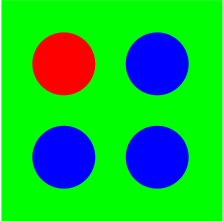
\includegraphics[width=0.4\linewidth]{fig/marker1.png}
	\caption{Marker 1.}
	\label{fig:mar1}
\end{figure}
For this marker we decided to use color segmentation as our approach. The points we extracted were the centers of the three blue circles.\par
We began by converting the image to HSV colour space, splitting its channels and looking at the hue channel as seen in figure \ref{fig:hue1}. We then took the hue value for the blue areas in the original marker as a reference. We used this value to compute a binary image showing only areas with a hue value very close to the desired blue one. The resulting binary image is shown in figure \ref{fig:bin1}. This isolated the the blue circles from the marker very nicely but left some noise from the blue background elements. To ignore this noise, we took advantage of the circles' shape. We found the contours in this binary image and the radius of their minimum enclosing circle. By comparing this radius to the contour's area, we got a value which quantitatively described the roundness of the contour. By selecting the three roundest contours in the binary image, we obtained the three circles in the marker as seen in figure \ref{fig:src1}.\par
We used this marker to test the simulated visual servoing system. In order for the robot to follow the marker's orientation, the three extracted points must be sorted in a consistent manner. To implement this, we first made the assumption that the points form a triangle whose longest side is always the same one. While this is not true for all out-of-plane rotations, it holds for all the projections in the provided sequences. Following this assumption, we used the point opposite the long side as the first element and used the cross product of the two short sides to sort the remaining two points clockwise.\par
This algorithm finds the points with high precision on each image in the provided sequences. It handles in-plane and out-of-plane rotations and scaling but the colors are somewhat sensitive to ambient light changes. A blue ball or similar in the background would also be very troublesome.\par
The color segmentation approach is appropriate for this problem due to the sharp colors on the marker. Our method for circle detection is also quite robust for this problem due to the fact that the circles are well isolated and that we know beforehand how many to look for.

\begin{figure}
	\centering
	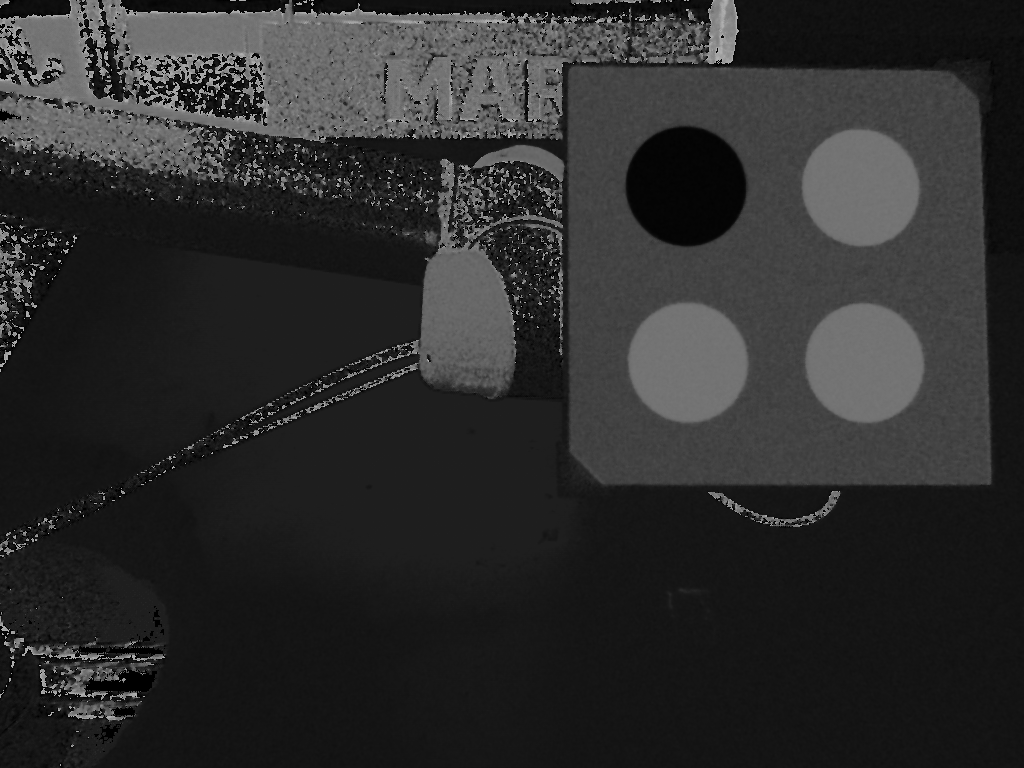
\includegraphics[width=0.7\linewidth]{fig/hue0-1.png}
	\caption{Hue channel of the first image in the color marker sequence.}
	\label{fig:hue1}
\end{figure}

\begin{figure}
	\centering
	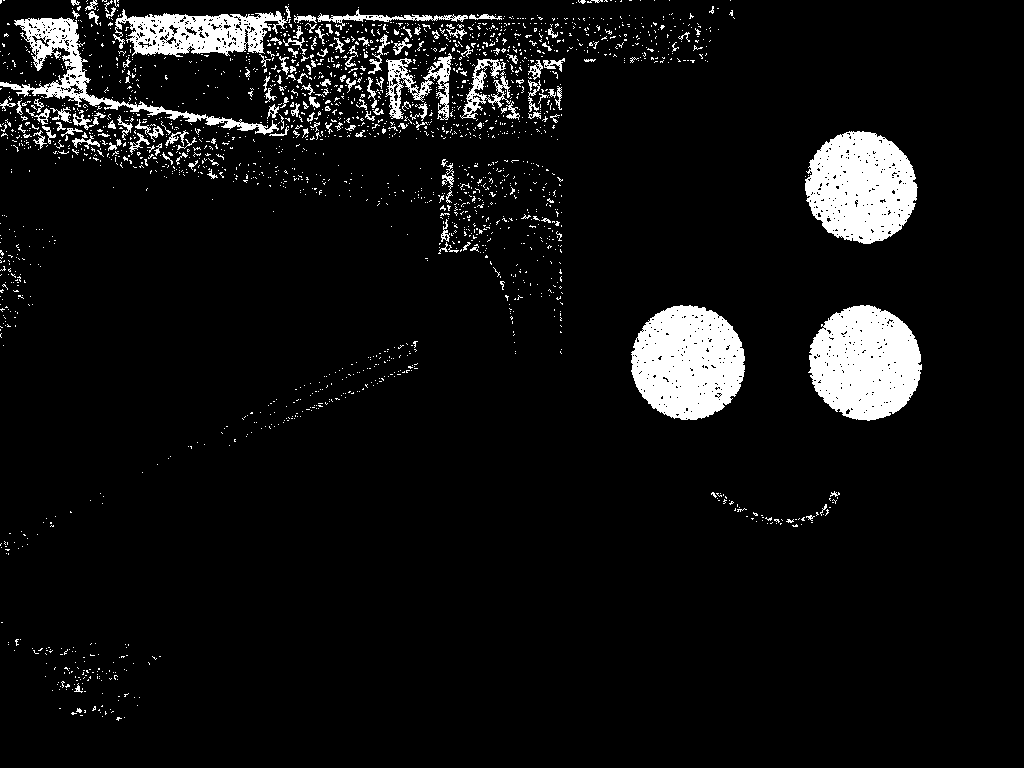
\includegraphics[width=0.7\linewidth]{fig/bin0-1.png}
	\caption{Figure \ref{fig:hue1} after hue thresholding.}
	\label{fig:bin1}
\end{figure}

\begin{figure}
	\centering
	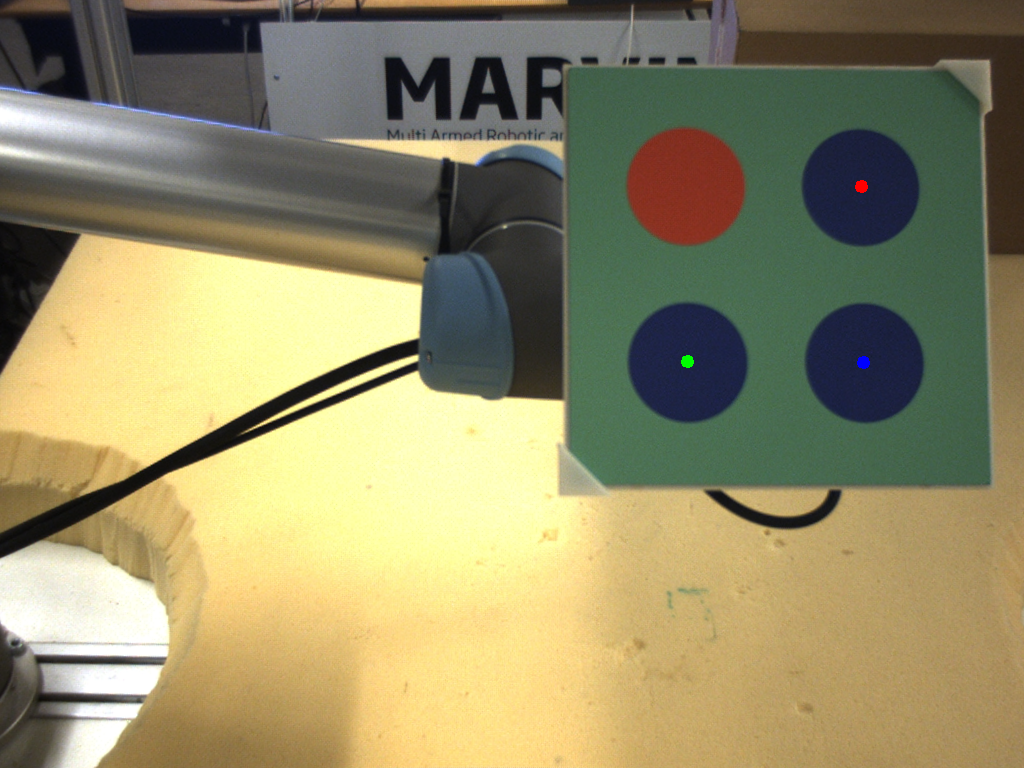
\includegraphics[width=0.7\linewidth]{fig/src0-1.png}
	\caption{Extracted points.}
	\label{fig:src1}
\end{figure}

\newpage
\subsection{Marker 2b}
\begin{figure}
	\centering
	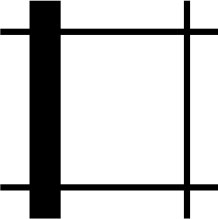
\includegraphics[width=0.4\linewidth]{fig/marker2b.png}
	\caption{Marker 2b.}
	\label{fig:mar2}
\end{figure}
For this marker we used the Hough transformation to find lines in the image. Our target points were the four corners of the white rectangle in the center of the marker.\par
We began by using the Canny algorithm to detect edges in the image as shown in figure \ref{fig:bin2}. We also used the Hough transform to detect the lines as shown in figure \ref{fig:lin2}. We dilated the edges as well as the lines and then combined them using logical AND as seen in figure \ref{fig:and2}. The resulting image shows the marker's lines relatively clearly with some background noise as well. From here we wanted to detect the innermost rectangle in the marker. We made the assumption that this rectangle is the largest one in this binary image. As for the first marker, we found the contours and this time their minimum enclosing rotated rectangle. This is quite a big approximation as it loses precision very quickly for out-of-plane rotations. To make sure we detect a rectangle, we compute a value which quantitatively describes how well the enclosing rectangle fits its corresponding contour. This value is given by \\
\centerline{\texttt{diff = abs( area - mu[i].m00 ) / area;}}\\
 and describes, in terms of percentage, how much of the bounding rectangle is not covered by the contour. This eliminates most contours apart from the white rectangles in the marker. Finally, we pick the largest remaining rectangle which is our desired one. See figure \ref{fig:src2}.\par
This algorithm finds the desired rectangle for each image in the provided sequences but its precision is subpar for out-of-plane rotations as seen in figure \ref{fig:err2}. The algorithm handles scaling and in-plane rotation but needs to find a closed contour around the desired rectangle. This makes it sensitive to sharp noise around the edges.\par
The Hough transformation is appropriate for this problem due to the long, sharp edges on the marker. We have chosen parameters for the line detection to maximize our chances to find the lines in the marker. We deal with the large number of false positives by ignoring the lines which don't correspond to edges in the image.\par

\begin{figure}
	\centering
	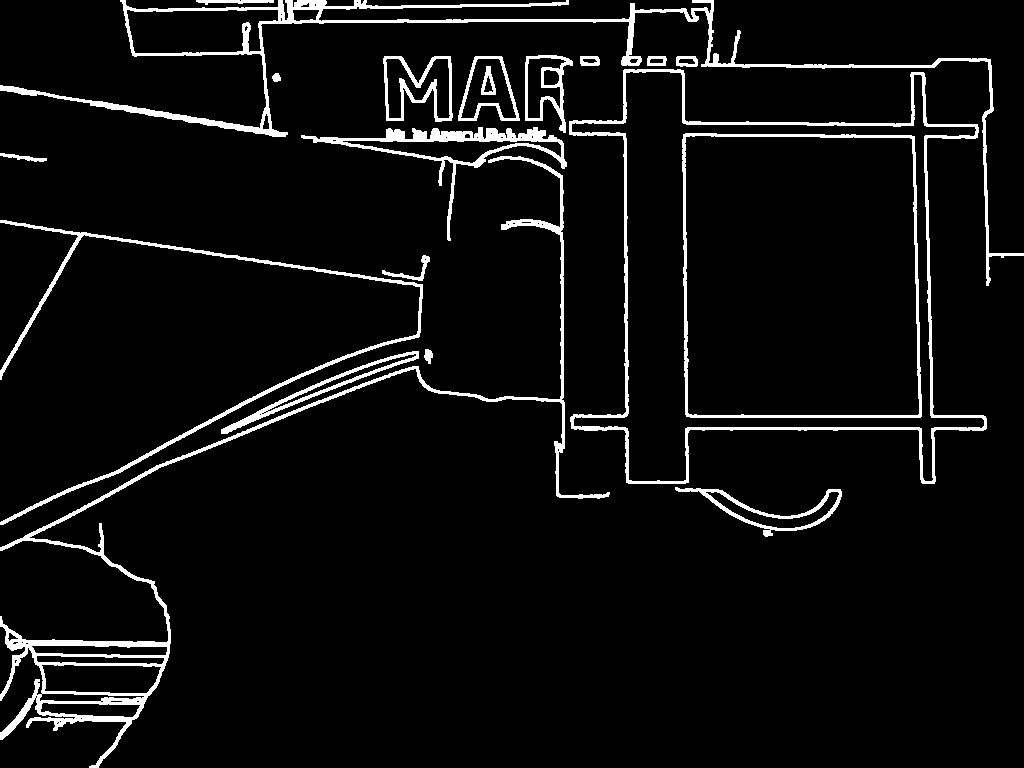
\includegraphics[width=0.7\linewidth]{fig/bin1-1.png}
	\caption{Edges from the first image in the thickline marker sequence.}
	\label{fig:bin2}
\end{figure}

\begin{figure}
	\centering
	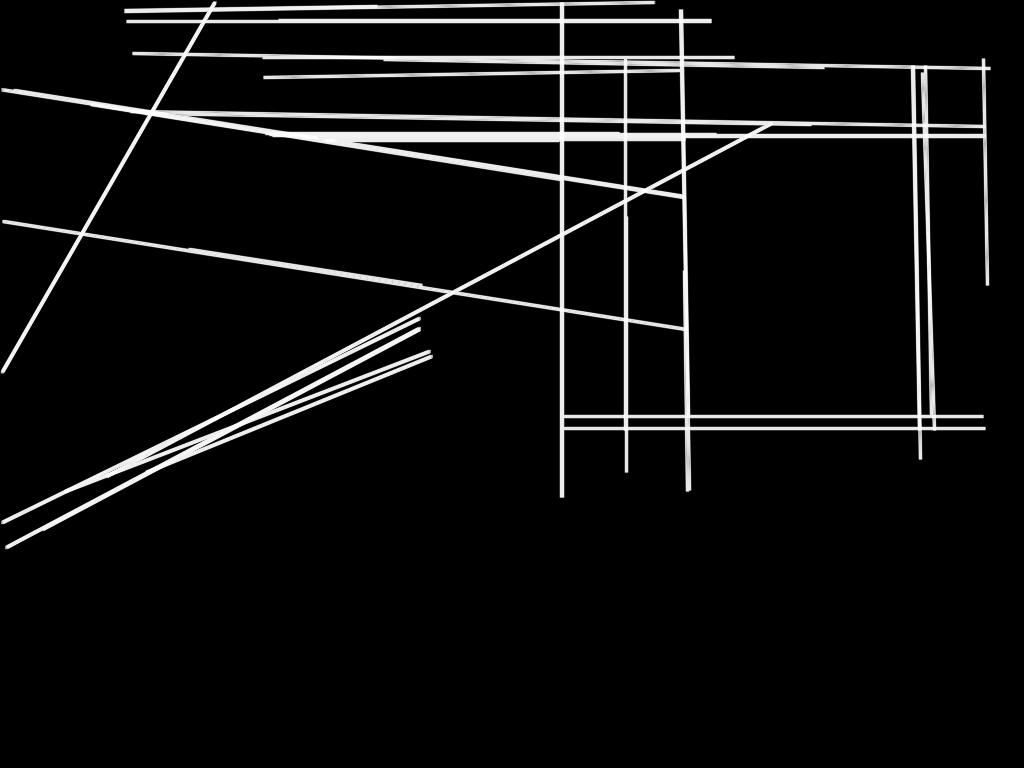
\includegraphics[width=0.7\linewidth]{fig/lin1-1.png}
	\caption{Hough lines from figure \ref{fig:bin2}.}
	\label{fig:lin2}
\end{figure}

\begin{figure}
	\centering
	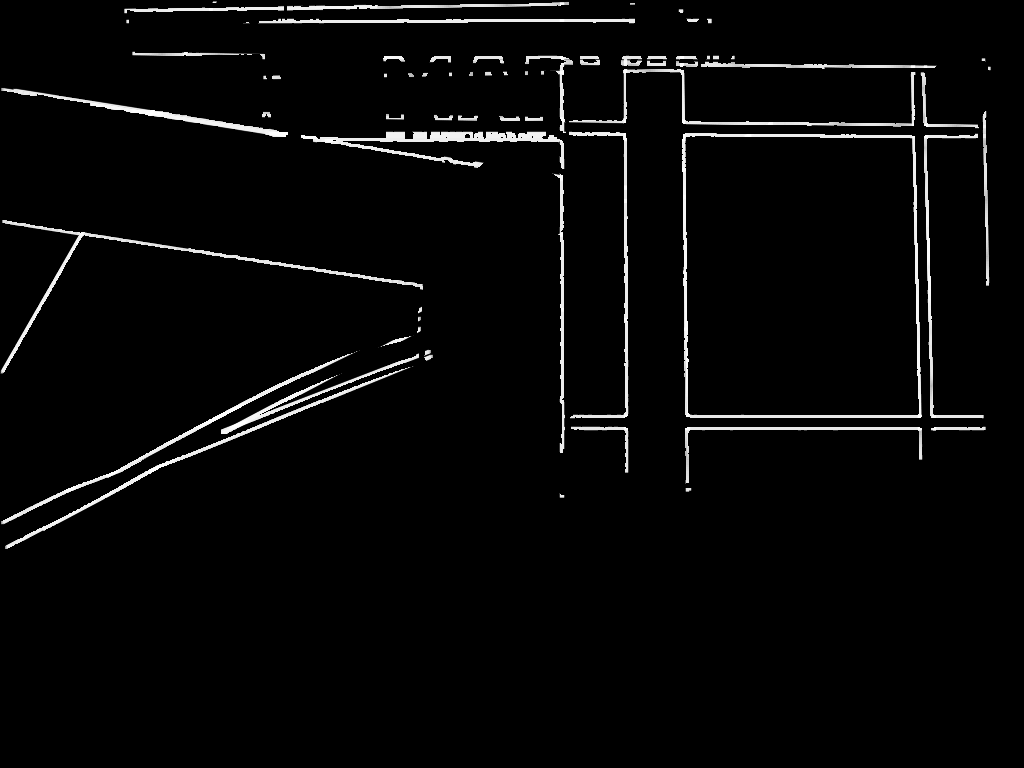
\includegraphics[width=0.7\linewidth]{fig/and1-1.png}
	\caption{Logical AND of figures \ref{fig:bin2} and \ref{fig:lin2}.}
	\label{fig:and2}
\end{figure}

\begin{figure}
	\centering
	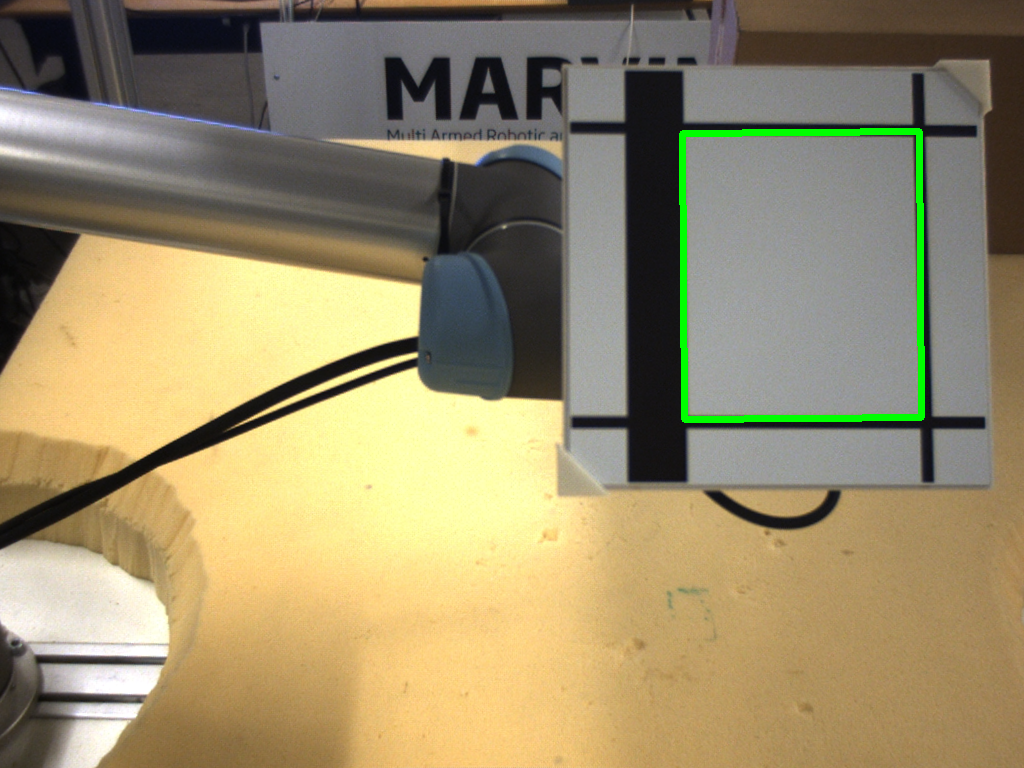
\includegraphics[width=0.7\linewidth]{fig/src1-1.png}
	\caption{Rectangle consisting of the four extracted points.}
	\label{fig:src2}
\end{figure}

\begin{figure}
	\centering
	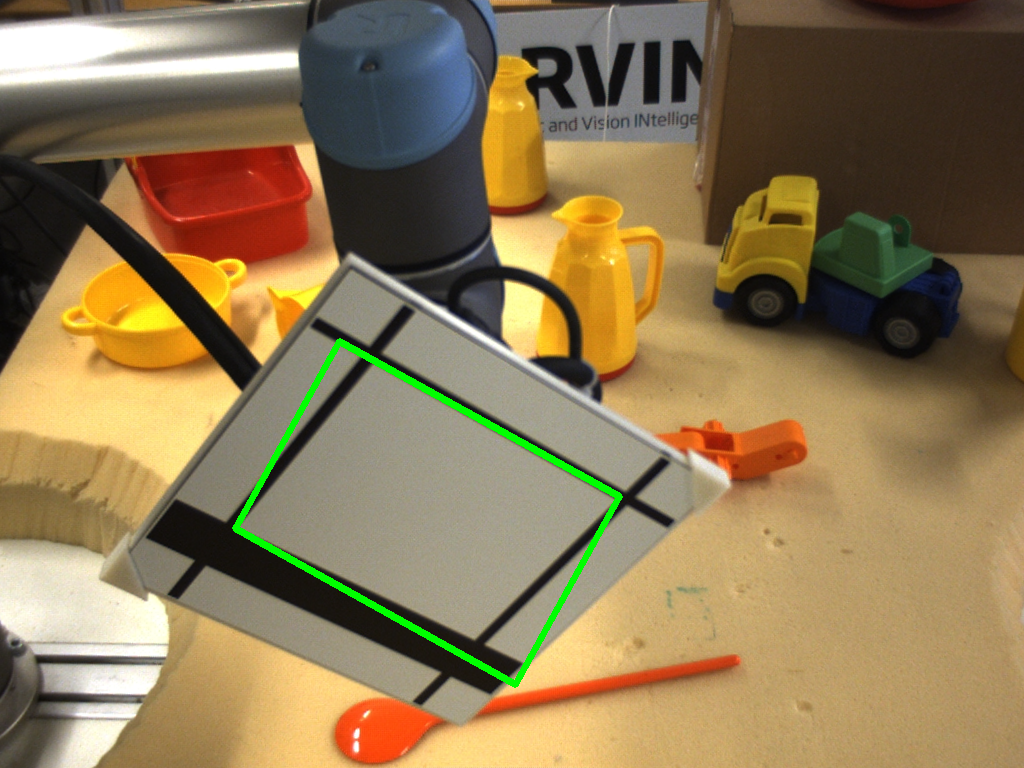
\includegraphics[width=0.7\linewidth]{fig/src1-63.png}
	\caption{Precision error for out-of-plane rotation.}
	\label{fig:err2}
\end{figure}

\clearpage
\section{Tracking points using image Jacobian}
We have implemented the algorithm for visual servoing in this part. For this part we selected specific marker points as described in the problem statement and used a mathematical camera model to get the image pixel coordinates of the points. Image recognition thus wasn't used in this part.

To compute joint updates we first needed to compose matrix $\boldsymbol{Z}_{image}$ as described in Robotics Notes:
\begin{align}
	\boldsymbol{Z}_{image}(\boldsymbol{q}) = \boldsymbol{J}_{image}\boldsymbol{S}(\boldsymbol{q})\boldsymbol{J}(\boldsymbol{q})\; 
\end{align}
where $\boldsymbol{J}(\boldsymbol{q})$ is the manipulator Jacobian. For its computation we used a function from RobWork library. $\boldsymbol{J}_{image}$ is the image Jacobian matrix. We implemented a function for its computation called \texttt{calculateImageJ} which can be found in the file \texttt{inverseKinematics.cpp}. We used a fixed value for the $z$ coordinate. Since we used the frame \texttt{cameraSim} to model the camera we set $z\, = \, -0.5$ for every function call. Finally the matrix $\boldsymbol{S}(\boldsymbol{q})$ was composed by inserting the transpose of the rotational matrix $\boldsymbol{R}_{base}^{tool}$ twice to its diagonal.

The next piece of information necessary to compute the joints updates is the difference or move of target points $\overrightarrow{\boldsymbol{dU}}_{image}$. We have programmed the function \texttt{calculate\_dUImage} to solve for $\overrightarrow{\boldsymbol{dU}}_{image}$.

Having the matrixes $\boldsymbol{Z}_{image}$ and $\overrightarrow{\boldsymbol{dU}}_{image}$ it was possible to solve for the joint positional update ${\boldsymbol{dq}}$ using the method of Linear Least Squares.

We adapted two equations from the robotics notes into single expression for ${\boldsymbol{dq}}$ computation:
\begin{align}
	\boldsymbol{dq} = \boldsymbol{Z}^T\left(\boldsymbol{Z}\boldsymbol{Z}^T\right)^{-1} \overrightarrow{\boldsymbol{dU}}_{image}
\end{align}
In this equation we used $\boldsymbol{Z}$ to denote $\boldsymbol{Z}_{image}$.
For solving this LSM problem we have implemented the function \texttt{compute\_dQ\_LSM} which can be found in \texttt{inverseKinematics.cpp}.

\texttt{algorithm2} is the function, where are all of the described functions are organized together to compute joint updates $\boldsymbol{dq}$ based on the manipulator state and the error in image coordinates $\overrightarrow{\boldsymbol{dU}}_{image}$.

We have implemented the $J_{image}$ and $\overrightarrow{\boldsymbol{dU}}_{image}$ composition in a scalable way, so the same functions can be used to track one or multiple target points.

The model of the robot manipulator has velocity limits on its joint movements, so it was necessary to check if the limits were satisfied before joint updates. We did so by measuring time for inverse kinematics computations $\tau_1$, subtracting this time from the workcell update period specified by $\Delta T \longleftrightarrow$ \texttt{deltaT} and finally we divided the update $\boldsymbol{dq}$ by the result of the subtraction. The velocity of joint movement is the result of the operation:
\begin{align}
	\boldsymbol{\dot{q}} = \frac{\boldsymbol{dq}}{dt} = \frac{\boldsymbol{dq}}{\Delta T\, -\, \tau_1}
\end{align}
By comparing the actual velocity with manipulator limits it was possible to find out if the limits are satisfied. If they aren't the algorithm simply saturates joint movement in order to hold all conditions. For comparison and saturation, the function \texttt{saturateDQ} was implemented.

In the following section we provide simulation results from tests of inverse kinematics.

\subsection{Simulation Tests}
During simulations, we recorded joint configurations, tool/camera frame position and orientation for $\texttt{deltaT} = 1000 ms$ and finally we performed tests for different values for \texttt{deltaT} in the range $50\, ms < \texttt{deltaT} < 1000\, ms$ and plotted maximum errors of 
$\overrightarrow{\boldsymbol{dU}}_{image}$

\subsubsection*{Slow Marker Sequence}
\begin{figure}[!htp]
	% Maximum length
	\subfloat[Tracking Single Point]
	{
		\label{fig:Slow1PointJoints}
		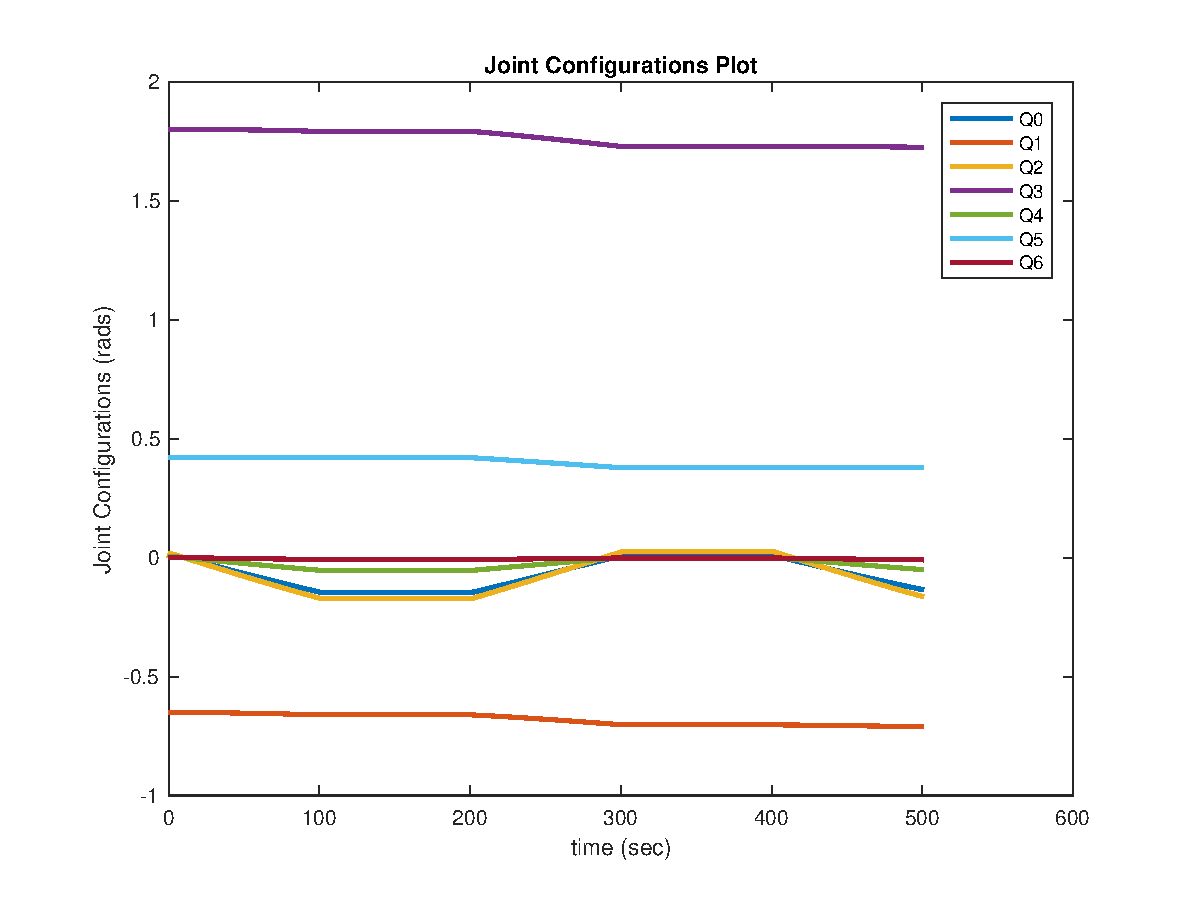
\includegraphics[width=0.49\linewidth]{fig/SlowSequence_joints_1_Targ_Pt.eps}
	}\hfill
	\subfloat[Tracking 3 Points]
	{
		\label{fig:Slow3PointsJoints}
		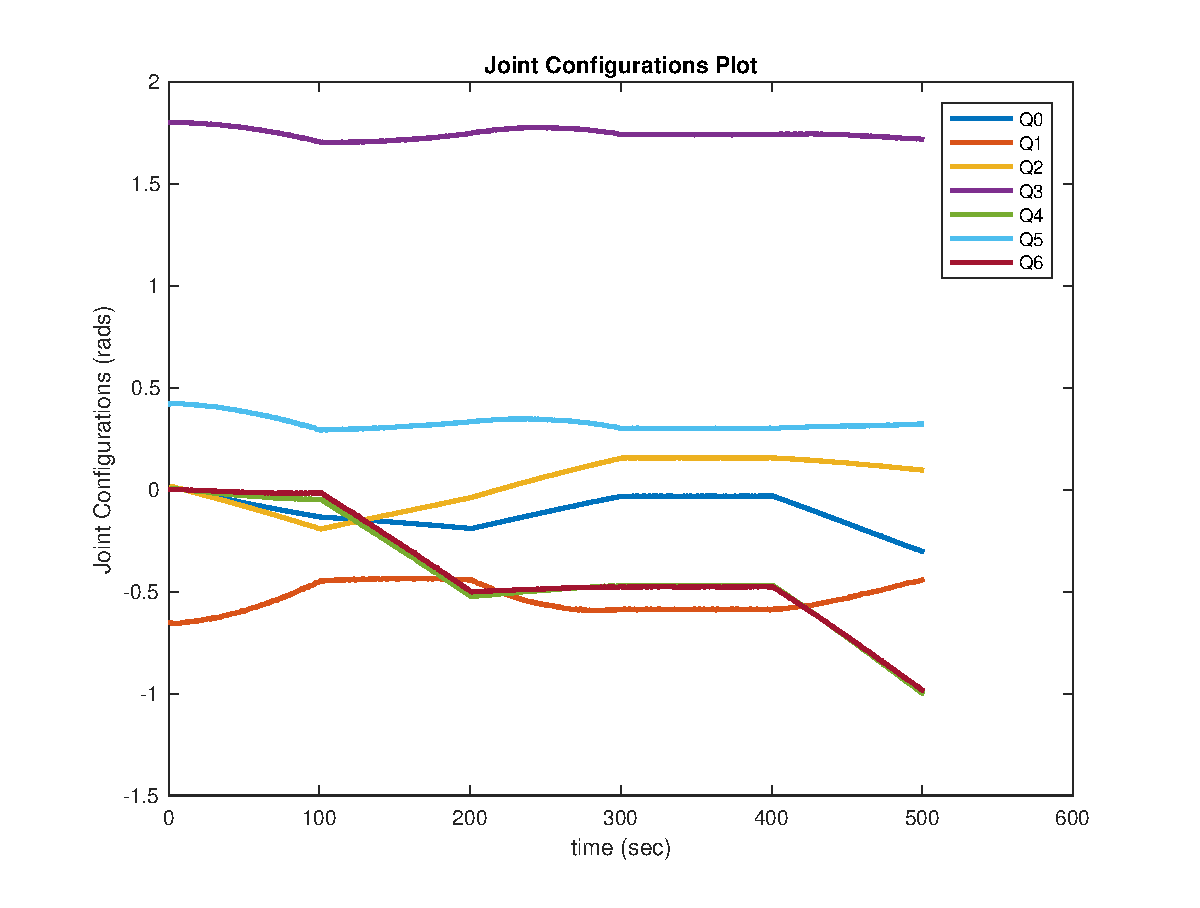
\includegraphics[width=0.49\linewidth]{fig/SlowSequence_joints_M_Targ_Pts.eps}
	}%
	\caption{Joint configurations}
	\label{fig:SlowSequenceJoints}
\end{figure}
There are differences between joint coordinates for tracking single and 3 target points in the graphs \ref{fig:Slow1PointJoints} and \ref{fig:Slow3PointsJoints}. The reason behind this is the following. When the manipulator is tracking a single point, it just follows its position. There is no orientation information about the marker when using a single tracking point. Whereas during following of 3 target points, the orientation of the marker gains an important role, as the manipulator is trying to rotate its tool/camera frame to align its position and orientation with the marker. 

\begin{figure}[!h]
	% Maximum length
	\subfloat[Tracking Single Point]
	{
		\label{fig:Slow1PointToolPose}
		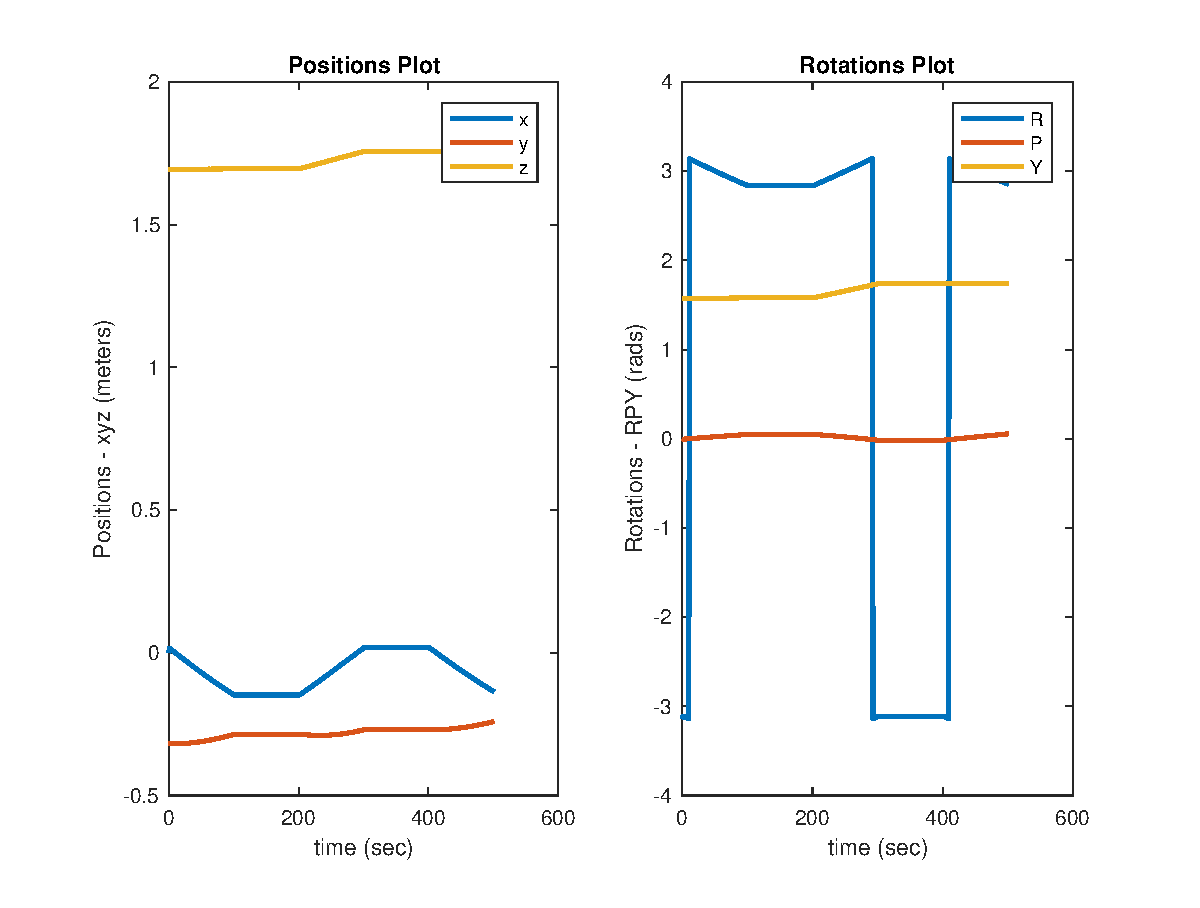
\includegraphics[width=0.49\linewidth]{fig/SlowSequence_tool_pose_1_Targ_Pt.eps}
	}\hfill
	\subfloat[Tracking 3 Points]
	{
		\label{fig:Slow3PointsToolPose}
		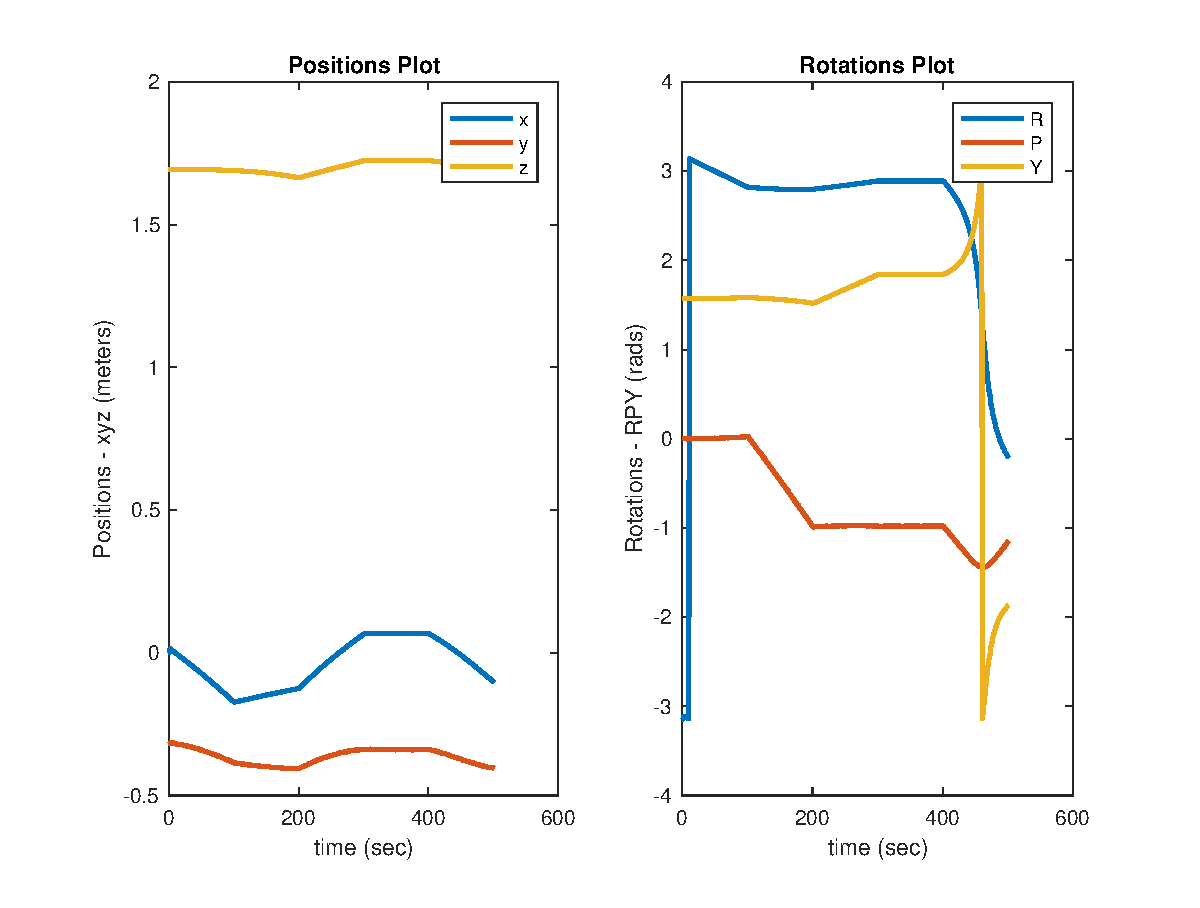
\includegraphics[width=0.49\linewidth]{fig/SlowSequence_tool_pose_M_Targ_Pts.eps}
	}%
	\caption{Tool pose transformations}
	\label{fig:SlowSequenceToolPose}
\end{figure}
In figure \ref{fig:Slow1PointToolPose} and \ref{fig:Slow3PointsToolPose} are apparent jumps in roll angle around $z$ axis. This however doesn't imply jumps in tool orientation. The abrupt jumps in the graphs were caused because of switching between angles of $-\pi$ and $\pi$ rad. In the real world, the change in orientation is small. The implementation of Robwork transformations probably keeps all orientation angles in the interval $ \langle -\pi, \; \pi \rangle $.

\vspace{0.5cm}
\begin{figure}
	\centering
	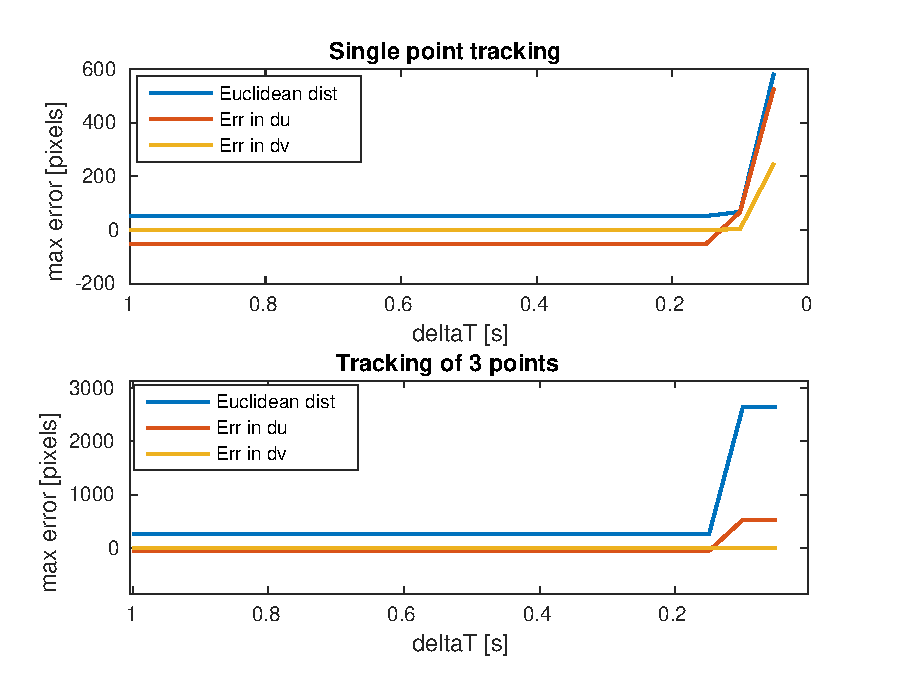
\includegraphics[width=0.7\linewidth]{fig/SlowSequence_errors.eps}
	\caption{Maximum errors during Slow Sequence Marker following}
	\label{fig:SlowSequence_errors}
\end{figure}

\vspace{0.5cm}
\textbf{Simulation for different $\Delta T$s} \\
\begin{figure}
	\centering
	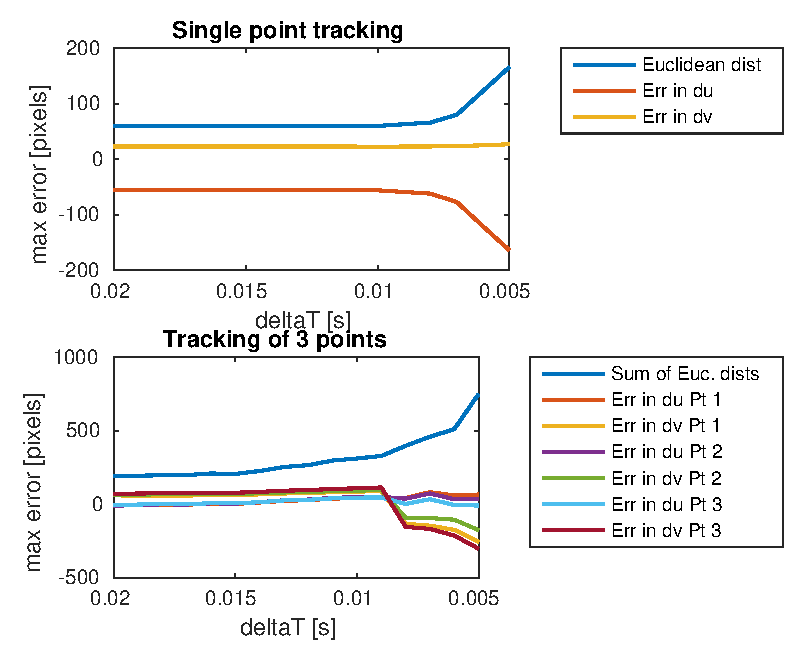
\includegraphics[width=0.7\linewidth]{fig/SlowSequence_low_dTs_errors.eps}
	\caption{Maximum errors during Slow Sequence Marker following}
	\label{fig:SlowSequence_low_dTs_errors}
\end{figure}

There are plotted maximum pixel errors on the figure \ref{fig:SlowSequence_errors}.

For timing purposes we used the C++ Chrono library, for taking time instant of the start of the computation of updates and the end instant. For differentiation of joint updates and subsequently getting of velocity, we used the difference of these two time stamps divided by the time left for the joints update. 

As you can see on figure \ref{fig:SlowSequence_errors} we didn't reach manipulator velocity limits in the interval $\Delta T \, \in \langle0.05, 1\rangle \, [s]$ as was described in the problem statement.

For this reason we lowered the interval to $\Delta T \, \in \langle0.005, 0.02\rangle \, [s]$. And in this case, there is an apparent increase in maximum errors for low $\Delta T$. The results are plotted in figure \ref{fig:SlowSequence_low_dTs_errors}.

Due to non-real-time OS, results might be different for each simulation and don't offer precise information. However for the purpose of the school exercise, we were able to limit joints speed velocities according to the problem statement.


\subsubsection*{Medium Marker Sequence}
The same problems and explanation apply for the Medium marker sequence. Joint coordinates and tool positions are plotted on the graphs \ref{fig:MediumSequenceJoints} and \ref{fig:MediumSequenceToolPose}. Only difference from Slow sequence is in the time axis. Due to faster and larger movements the time span is shorter.
\begin{figure}[!htp]
	% Maximum length
	\subfloat[Tracking Single Point]
	{
		\label{fig:Medium1PointJoints}
		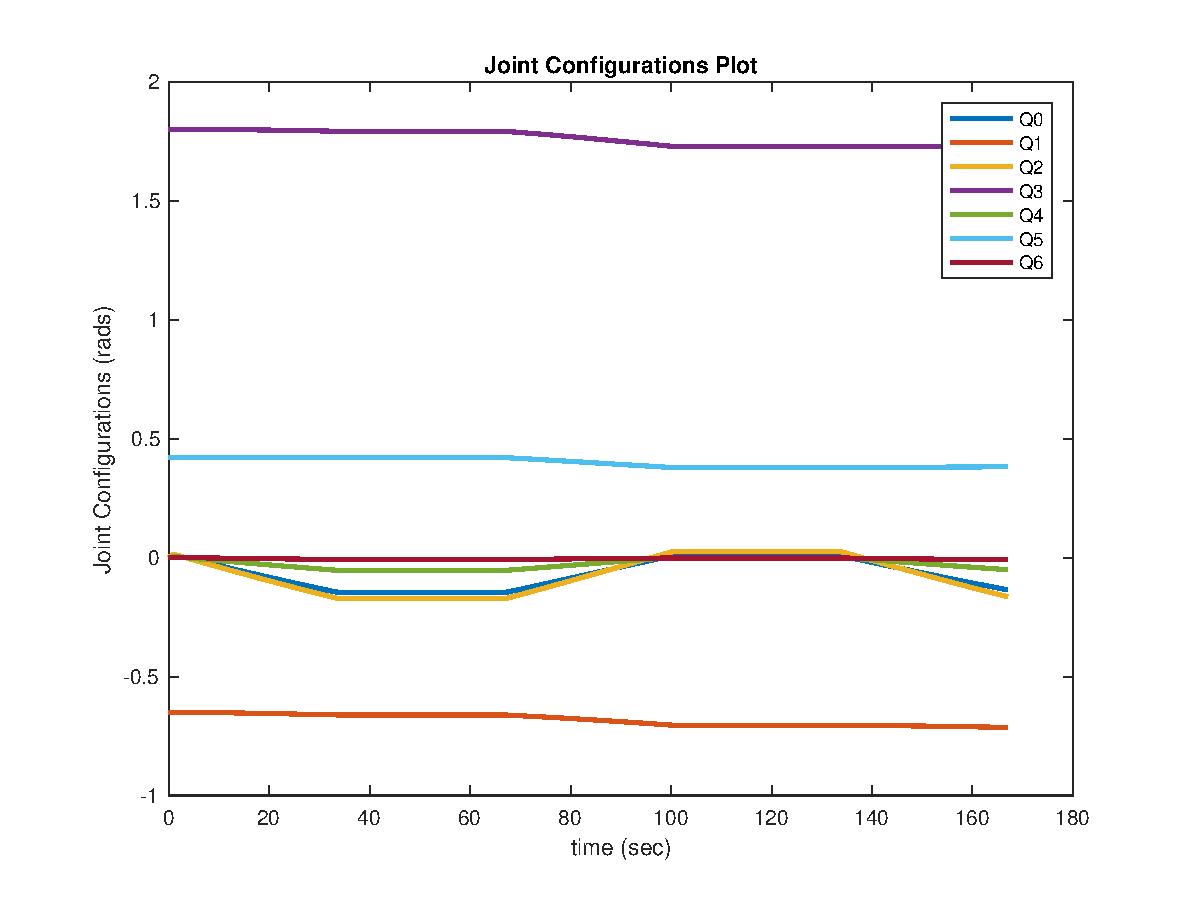
\includegraphics[width=0.49\linewidth]{fig/MediumSequence_joints_1_Targ_Pt.eps}
	}\hfill
	\subfloat[Tracking 3 Points]
	{
		\label{fig:Medium3PointsJoints}
		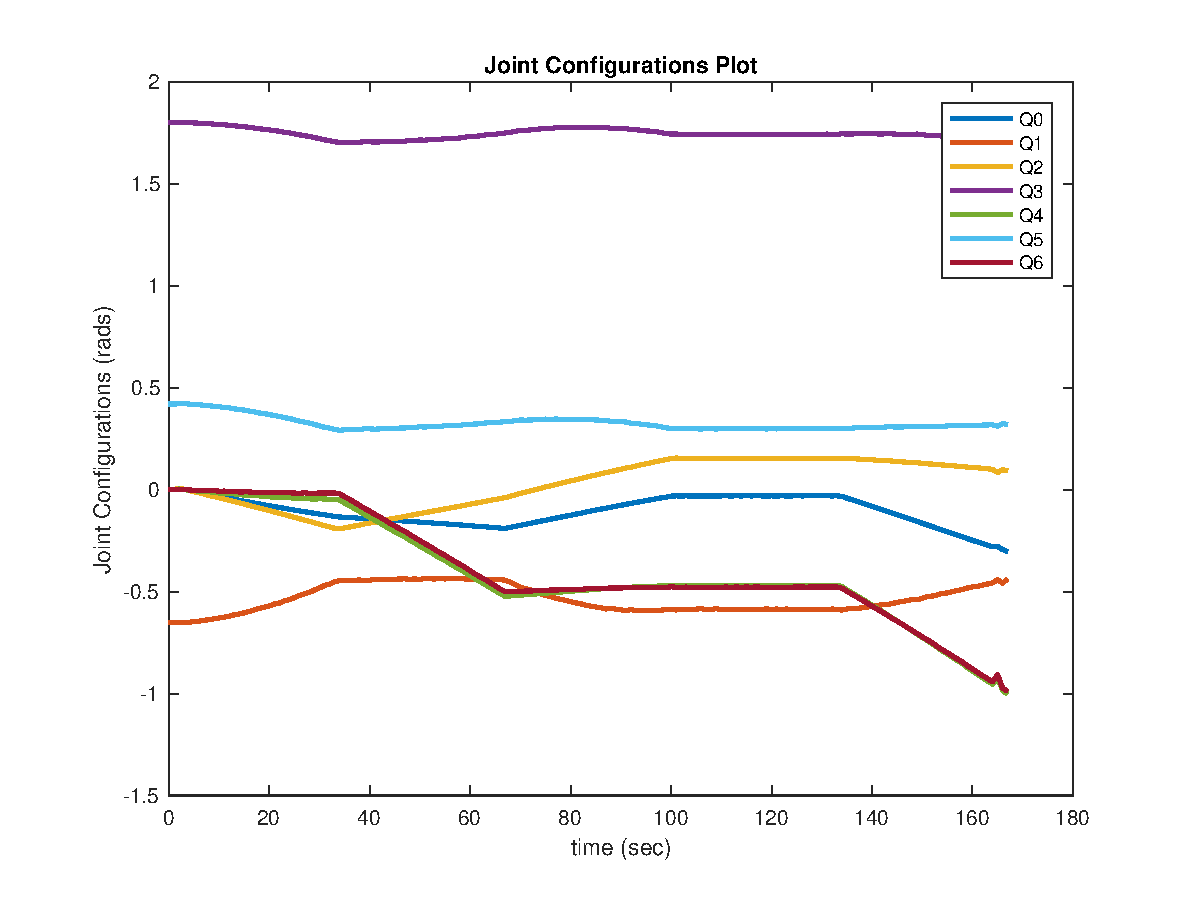
\includegraphics[width=0.49\linewidth]{fig/MediumSequence_joints_M_Targ_Pts.eps}
	}%
	\caption{Joint configurations}
	\label{fig:MediumSequenceJoints}
\end{figure}

\begin{figure}[!htp]
	% Maximum length
	\subfloat[Tracking Single Point]
	{
		\label{fig:Medium1PointToolPose}
		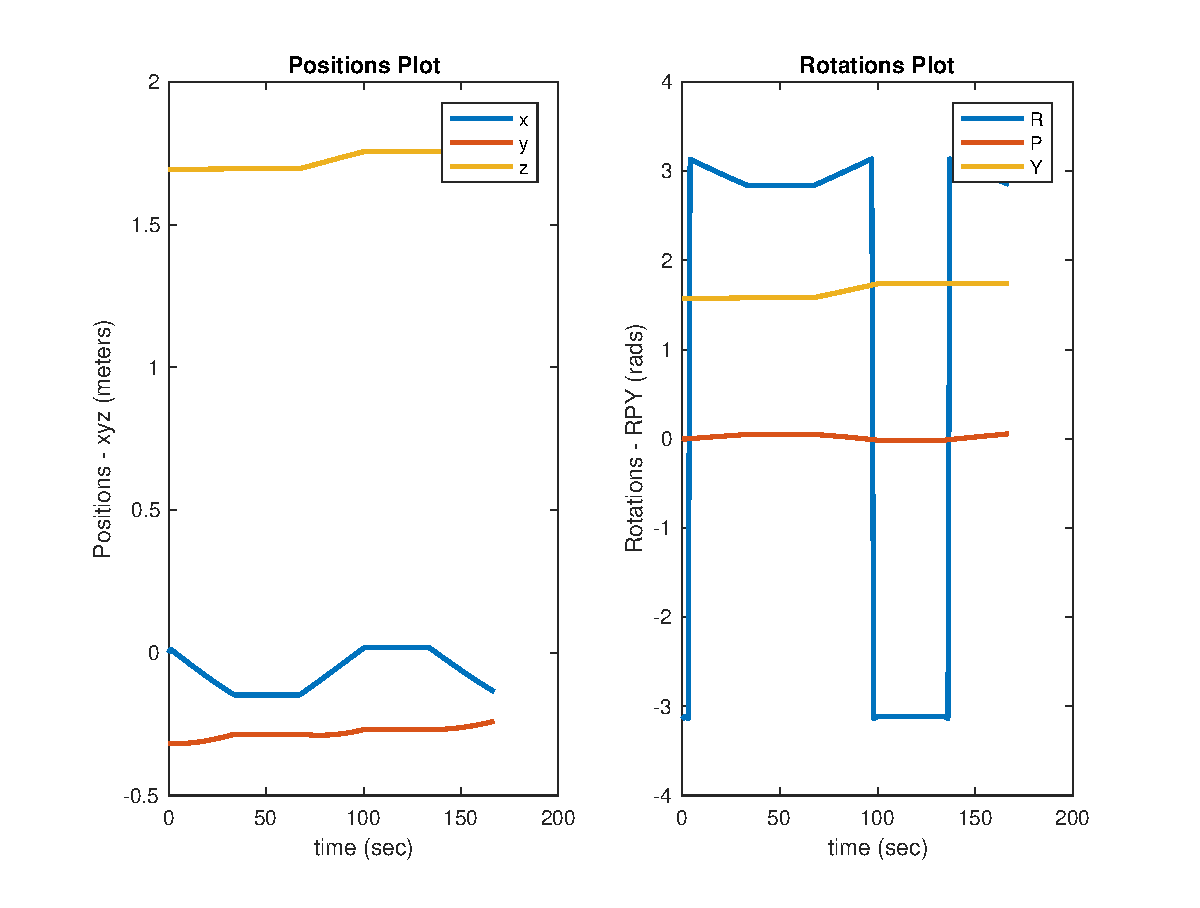
\includegraphics[width=0.49\linewidth]{fig/MediumSequence_tool_pose_1_Targ_Pt.eps}
	}\hfill
	\subfloat[Tracking 3 Points]
	{
		\label{fig:MediumPointsToolPose}
		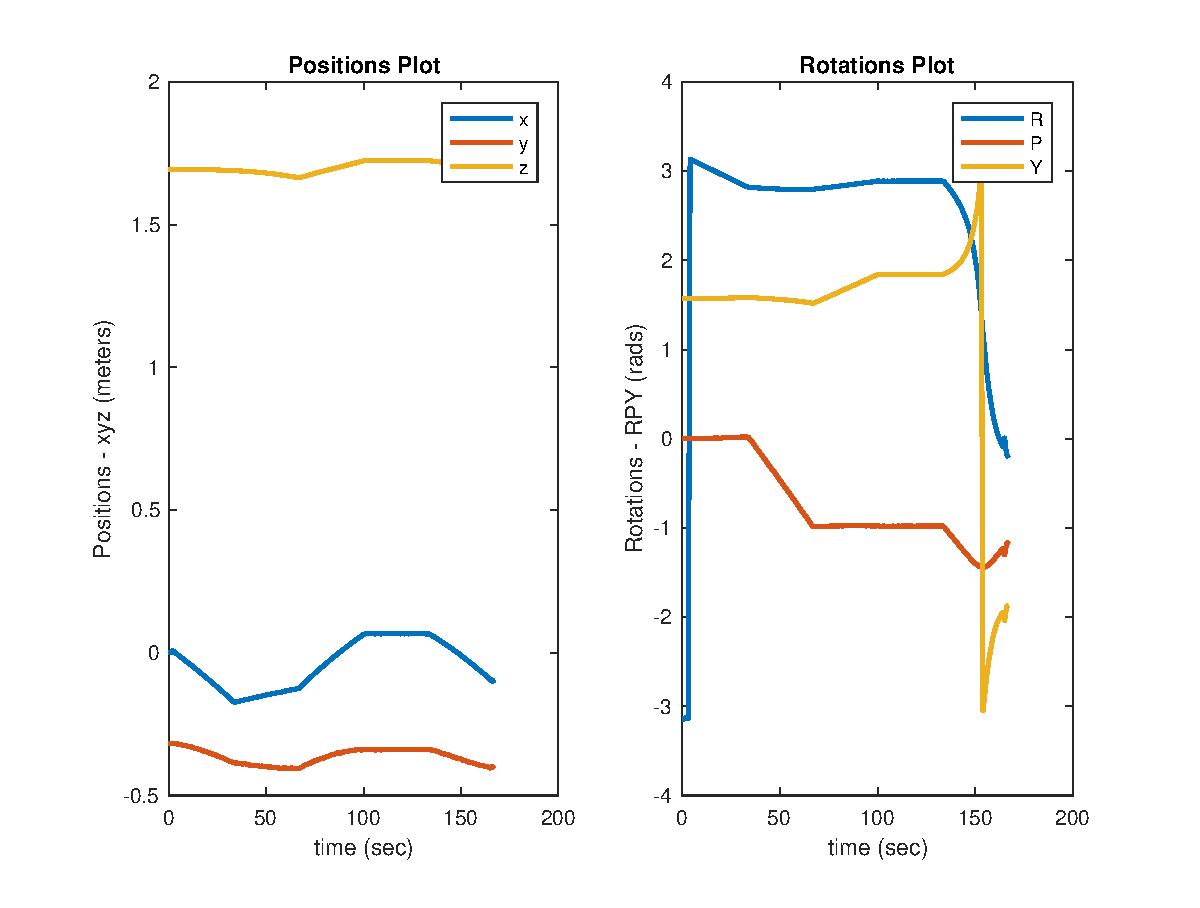
\includegraphics[width=0.49\linewidth]{fig/MediumSequence_tool_pose_M_Targ_Pts.eps}
	}%
	\caption{Tool pose transformations}
	\label{fig:MediumSequenceToolPose}
\end{figure}

\vspace{0.5cm}
\textbf{Simulation for different $\Delta T$s} \\
\begin{figure}
	\centering
	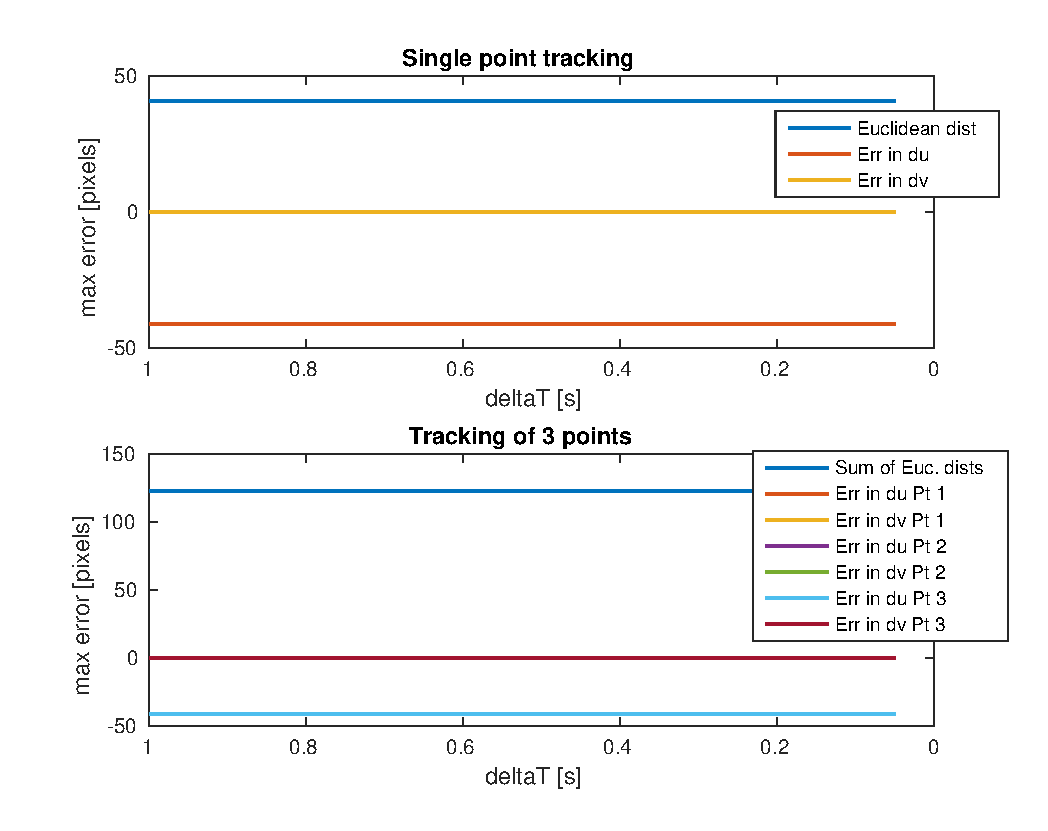
\includegraphics[width=0.7\linewidth]{fig/MediumSequence_errors.eps}
	\caption{Maximum errors during Medium Sequence Marker following}
	\label{fig:MediumSequence_errors}
\end{figure}
\begin{figure}
	\centering
	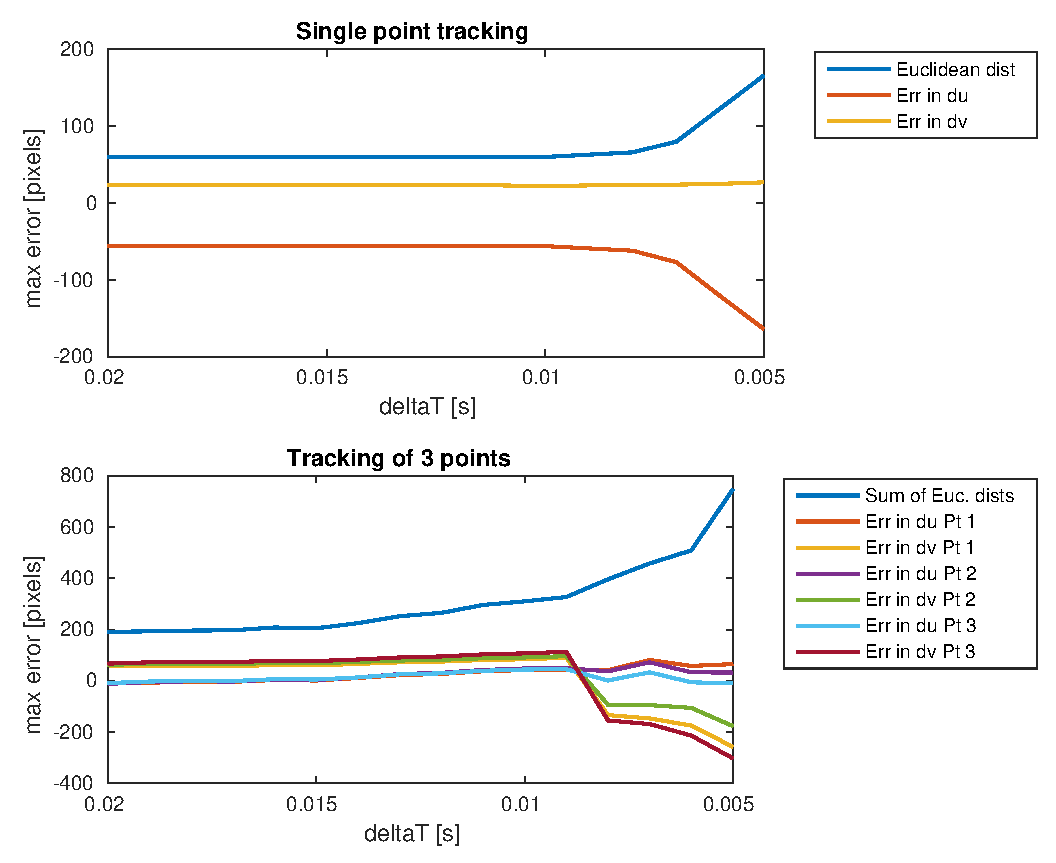
\includegraphics[width=0.7\linewidth]{fig/MediumSequence_low_dTs_errors.eps}
	\caption{Maximum errors during Medium Sequence Marker following}
	\label{fig:MediumSequence_low_dTs_errors}
\end{figure}
There are plotted maximum pixel errors on figure \ref{fig:MediumSequence_errors}. Again, we didn't reach the manipulator's velocity limits in the original interval. Results after lowering the interval of $\Delta T$ are plotted in figure \ref{fig:MediumSequence_low_dTs_errors}.

We have to state the same as for the preceding test. All timing tests were performed on a regular laptop PC, running non-real time operating system. So results from another tests can differ.

\subsubsection*{Fast Marker Sequence}
Joint coordinates and tool positions are plotted on graphs \ref{fig:FastSequenceJoints} and \ref{fig:FastSequenceToolPose}. The span of the time axis is again shorter.

\begin{figure}[!htp]
	% Maximum length
	\subfloat[Tracking Single Point]
	{
		\label{fig:Fast1PointJoints}
		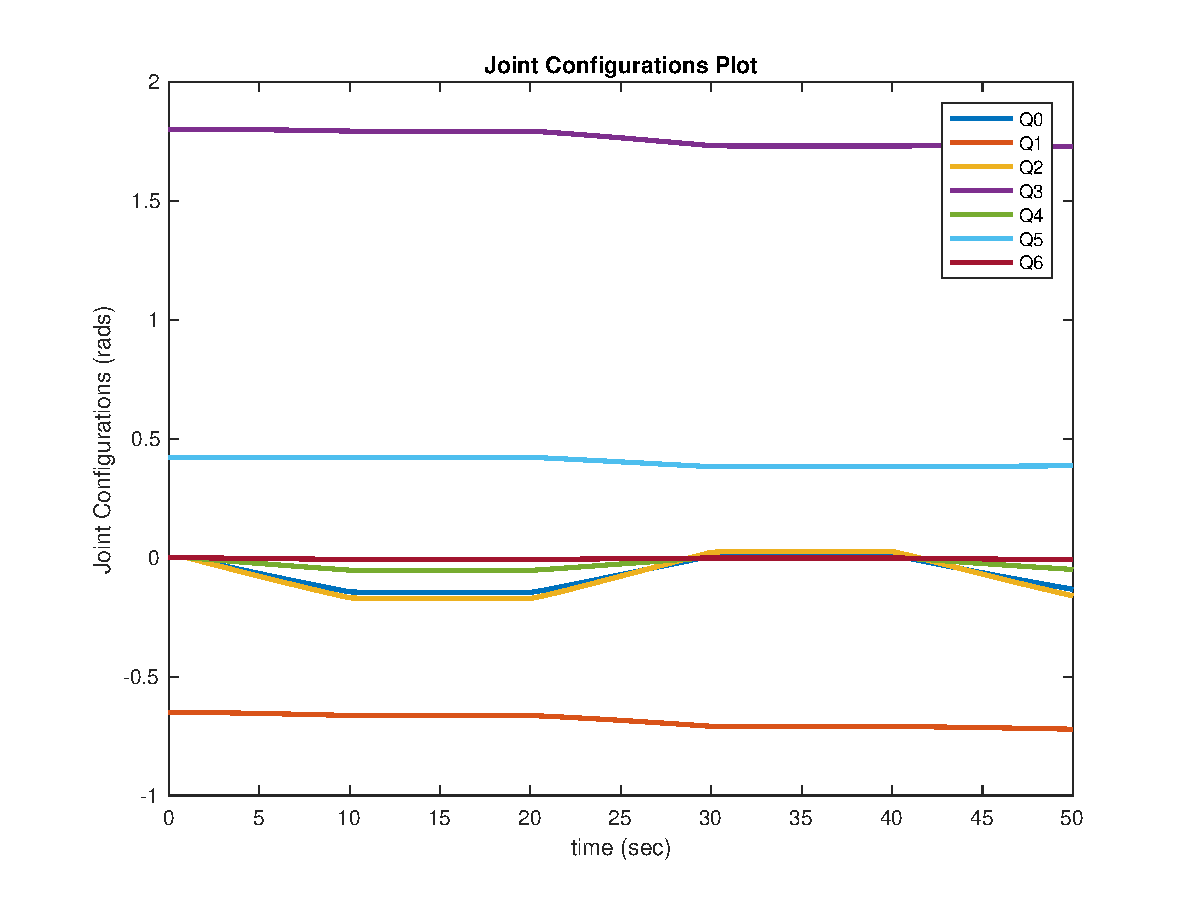
\includegraphics[width=0.49\linewidth]{fig/FastSequence_joints_1_Targ_Pt.eps}
	}\hfill
	\subfloat[Tracking 3 Points]
	{
		\label{fig:Fast3PointsJoints}
		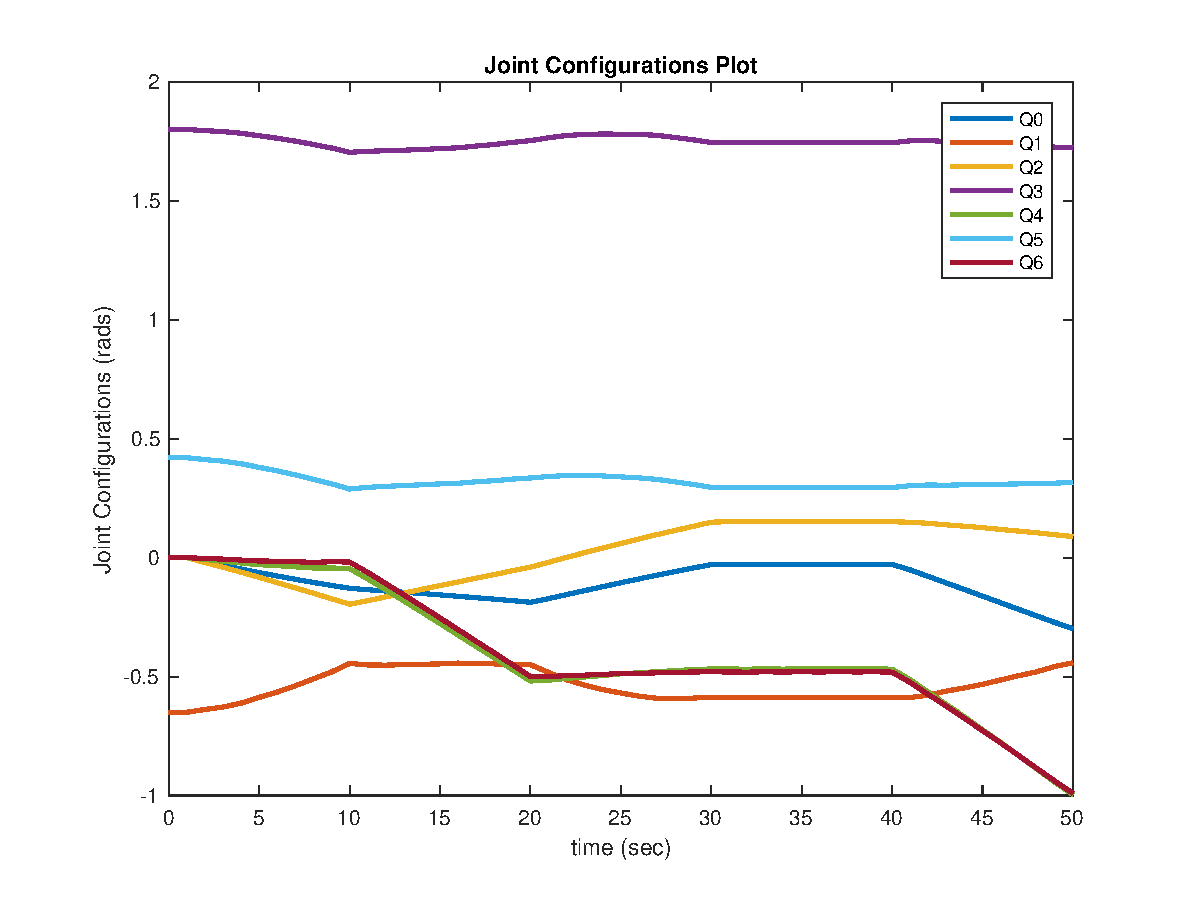
\includegraphics[width=0.49\linewidth]{fig/FastSequence_joints_M_Targ_Pts.eps}
	}%
	\caption{Joint configurations}
	\label{fig:FastSequenceJoints}
\end{figure}

\begin{figure}[!htp]
	% Maximum length
	\subfloat[Tracking Single Point]
	{
		\label{fig:Fast1PointToolPose}
		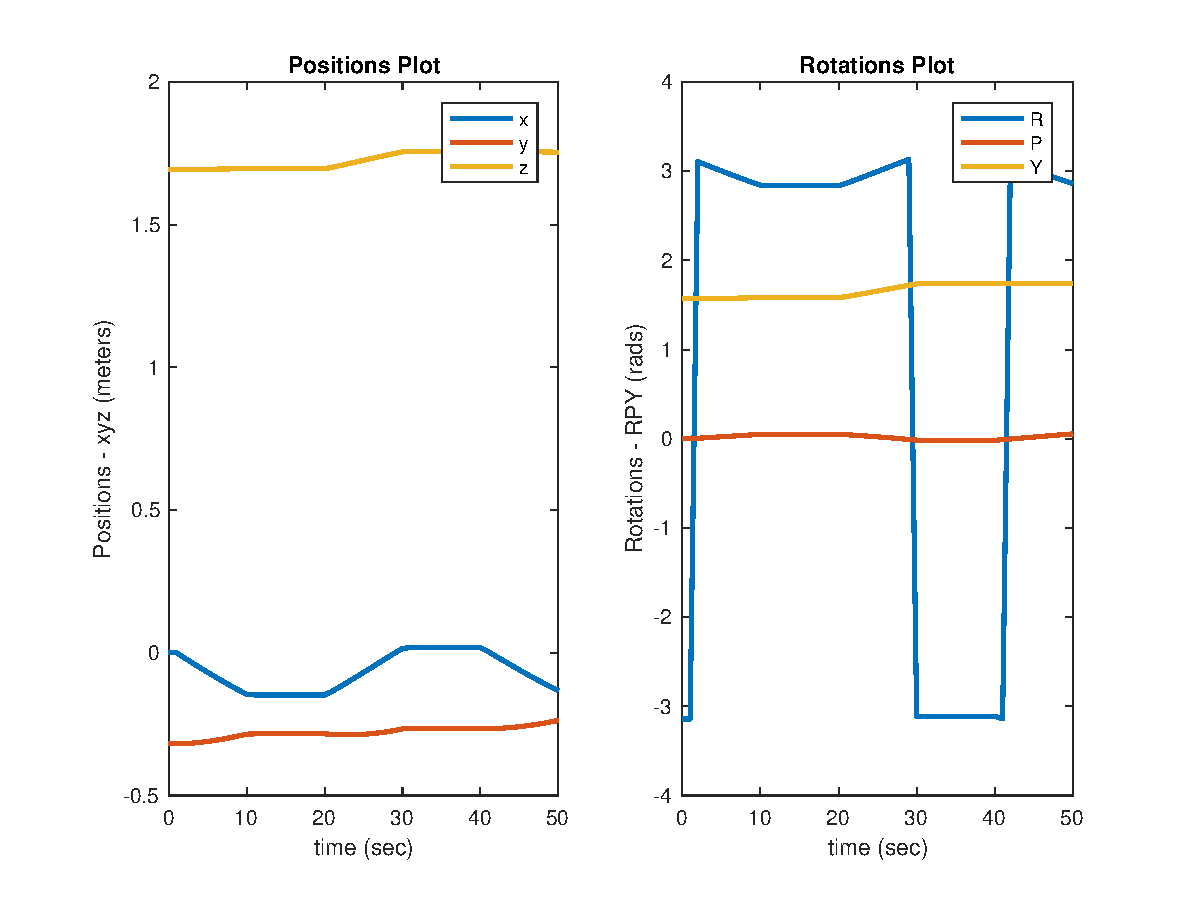
\includegraphics[width=0.49\linewidth]{fig/FastSequence_tool_pose_1_Targ_Pt.eps}
	}\hfill
	\subfloat[Tracking 3 Points]
	{
		\label{fig:FastPointsToolPose}
		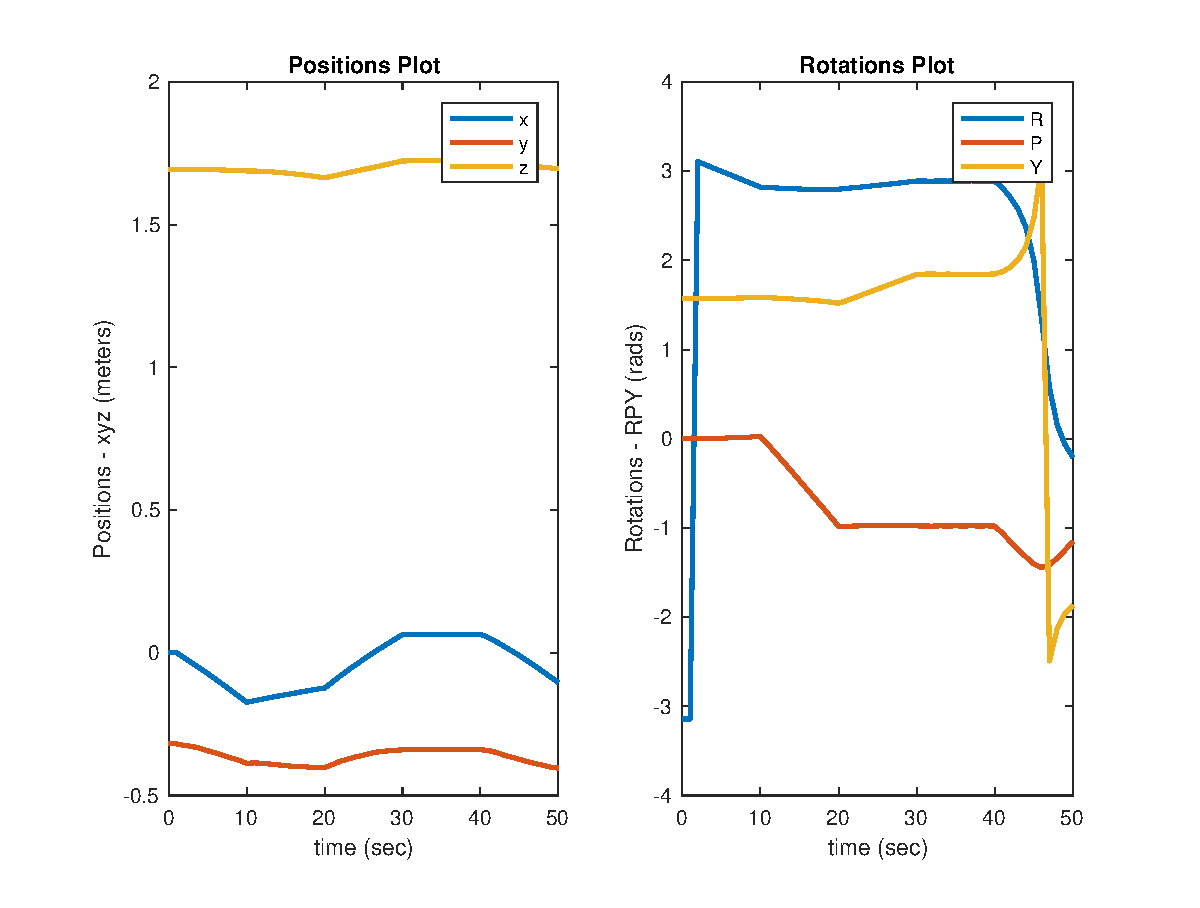
\includegraphics[width=0.49\linewidth]{fig/FastSequence_tool_pose_M_Targ_Pts.eps}
	}%
	\caption{Tool pose transformations}
	\label{fig:FastSequenceToolPose}
\end{figure}

\vspace{0.5cm}
\textbf{Simulation for different $\Delta T$s} \\
\begin{figure}
	\centering
	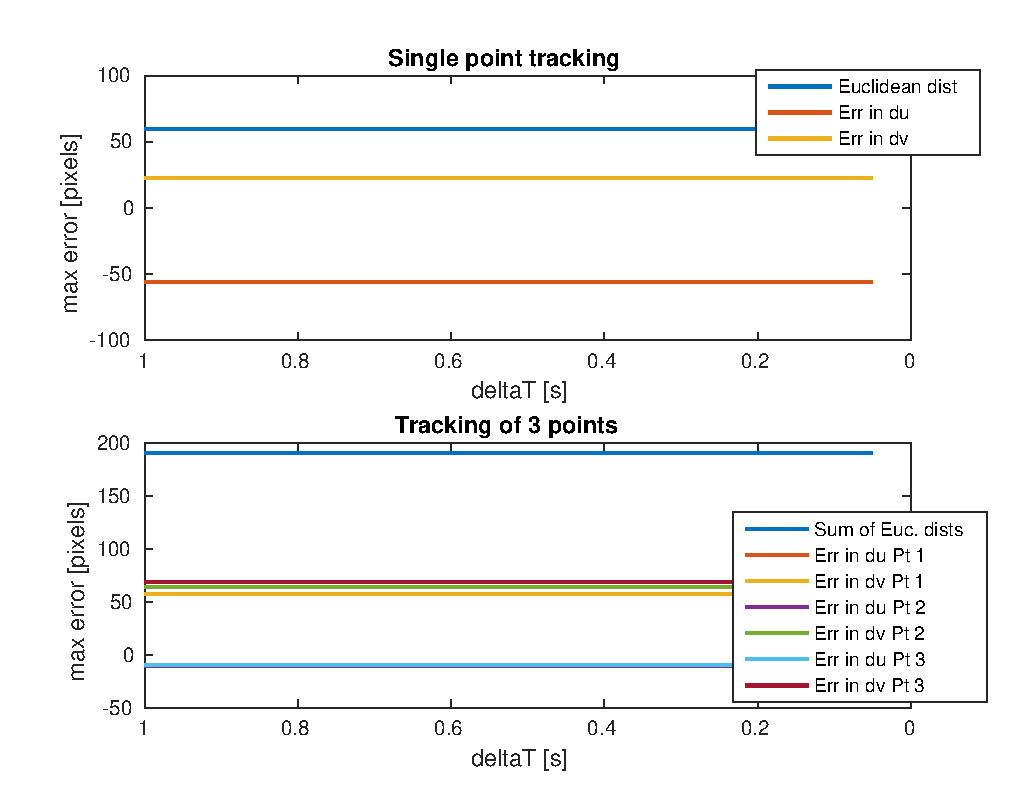
\includegraphics[width=0.7\linewidth]{fig/FastSequence_errors.eps}
	\caption{Maximum errors during Fast Sequence Marker following}
	\label{fig:FastSequence_errors}
\end{figure}

\begin{figure}
	\centering
	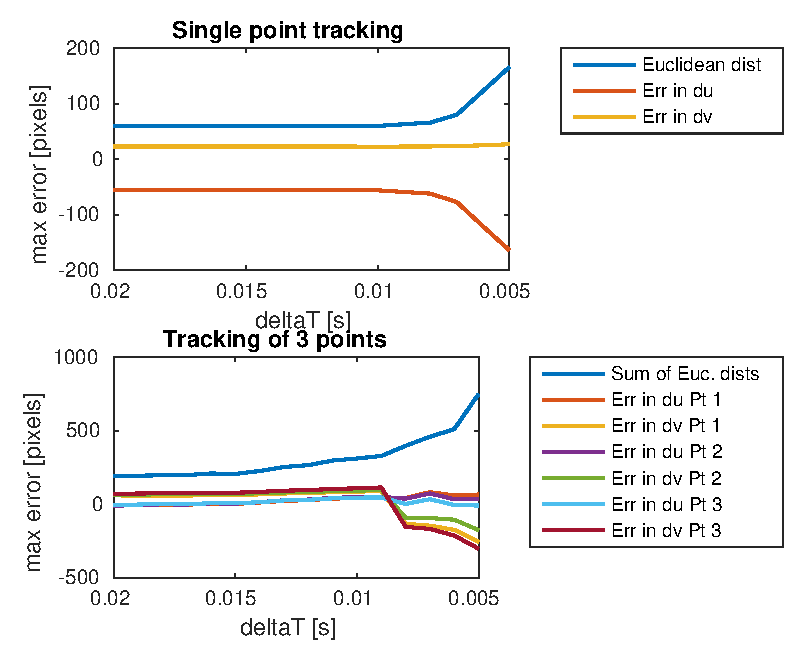
\includegraphics[width=0.7\linewidth]{fig/FastSequence_low_dTs_errors.eps}
	\caption{Maximum errors during Fast Sequence Marker following}
	\label{fig:FastSequence_low_dTs_errors}
\end{figure}

There are plotted maximum pixel errors on figure \ref{fig:FastSequence_errors} for the original interval. Results from simulations for the lower interval are plotted on figure \ref{fig:FastSequence_low_dTs_errors}.

\subsubsection*{Conclusion for different speed sequences}
Even though timing and velocity computation during test simulations wasn't precise due to non-realtime of the OS, we can conclude some final facts. 
The manipulator was able to follow the marker for each sequence with \texttt{deltaT} $ >\, 0.01 s$. The reason behind these results is probably the very short time needed for inverse kinematics computations. We found them to be in the order of microseconds, whereas simulation were performed for $\Delta T$s which were an order of magnitude larger (milliseconds). These results will be also different when simulated on a different computer.

\clearpage
\section{Combining feature extraction and tracking} 
For the last part of the project we have chosen Marker 1 for image recognition. Image recognition was integrated into the Robwork project. All these image recognition function are in the file \texttt{marker1.cpp}. For proper tracking of multiple points, it was necessary to sort the detected points in a consistent order for every detection.

After performing several tests we have found that the recognition time varies among different machines. The average time for one of our computer was around 30 ms whereas on the second one it was just around 25 ms.

For further plots we have chosen a value for \texttt{deltaT} which did not cause any problems during following. Thehe second one is too short and the unsaturated joints velocities are larger than their limits.

\begin{figure}[!htp]
	% Maximum length
	\subfloat[Tracking Single Point]
	{
		\label{fig:SlowSequence_dT50_1Pt_following_error_vs_time}
		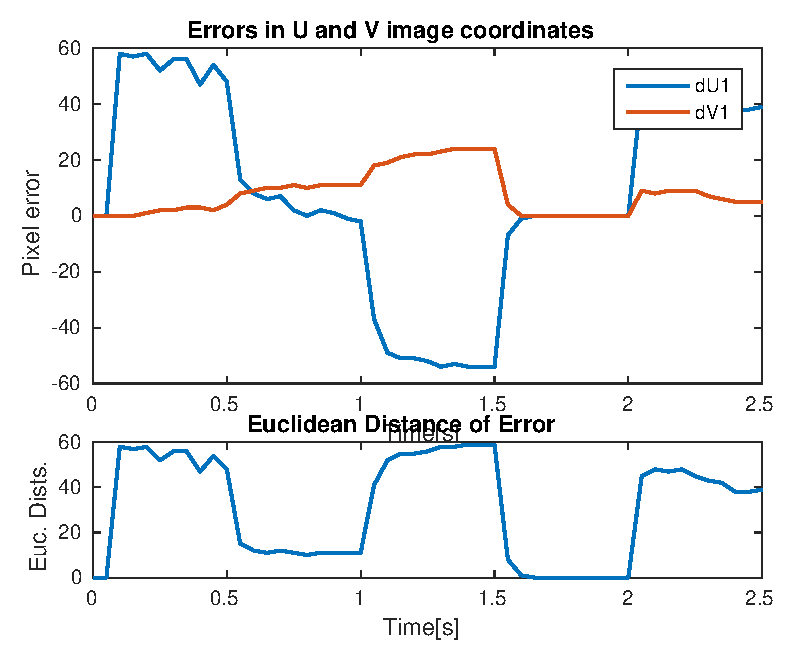
\includegraphics[width=0.49\linewidth]{fig/SlowSequence_dT50_1Pt_following_error_vs_time.eps}
	}\hfill
	\subfloat[Tracking 3 Points]
	{
		\label{fig:SlowSequence_dT50_MPt_following_error_vs_time}
		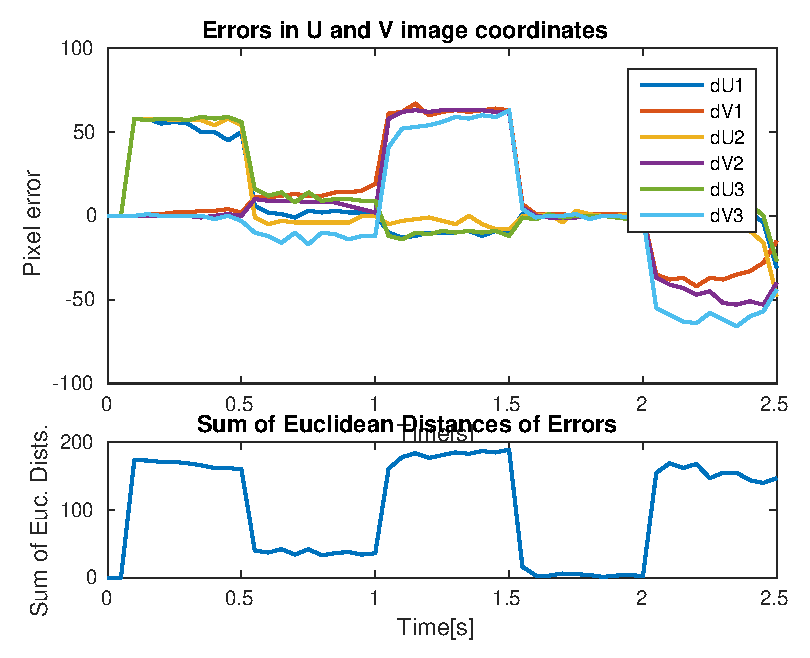
\includegraphics[width=0.49\linewidth]{fig/SlowSequence_dT50_MPt_following_error_vs_time.eps}
	}%
	\caption{Slow Sequence, \texttt{deltaT = 50} ms}
	\label{fig:SlowSequence_dT50_following_error_vs_time}
\end{figure}
\begin{figure}[!htp]
	% Maximum length
	\subfloat[Tracking Single Point]
	{
		\label{fig:SlowSequence_dT35_1Pt_following_error_vs_time}
		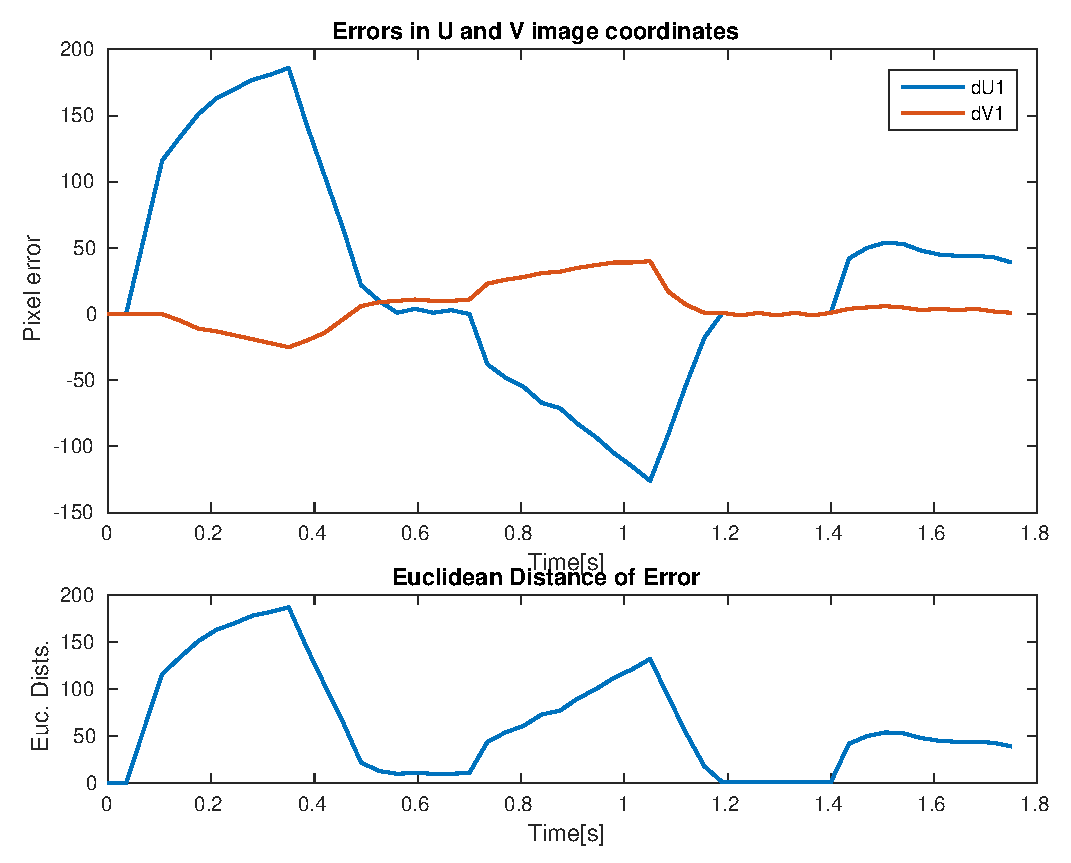
\includegraphics[width=0.49\linewidth]{fig/SlowSequence_dT35_1Pt_following_error_vs_time.eps}
	}\hfill
	\subfloat[Tracking 3 Points]
	{
		\label{fig:SlowSequence_dT35_MPt_following_error_vs_time}
		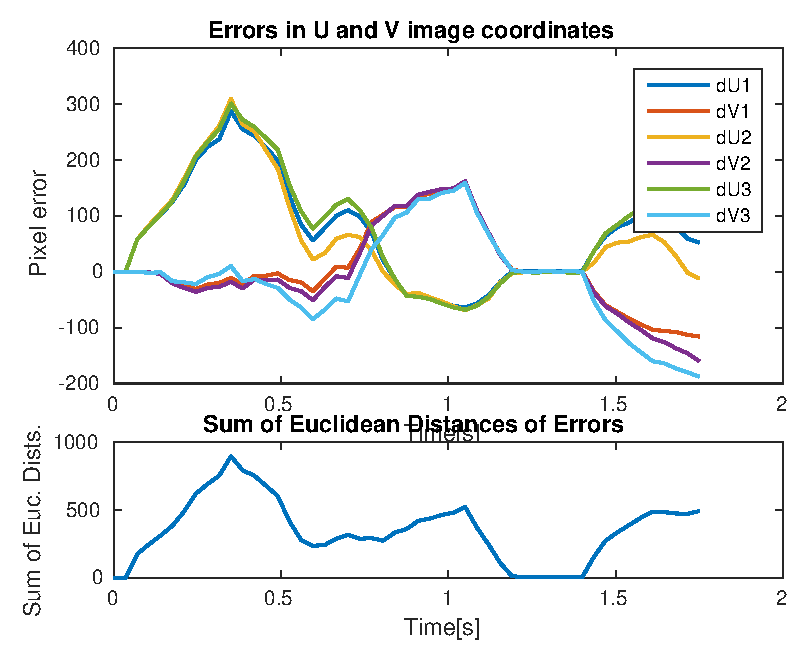
\includegraphics[width=0.49\linewidth]{fig/SlowSequence_dT35_MPt_following_error_vs_time.eps}
	}%
	\caption{Slow Sequence, \texttt{deltaT = 35} ms}
	\label{fig:SlowSequence_dT35_following_error_vs_time}
\end{figure}
It is possible to see, that the tracking error is generally larger on figure \ref{fig:SlowSequence_dT35_following_error_vs_time} than on figure \ref{fig:SlowSequence_dT50_following_error_vs_time}. The reason is that the velocity limits were violated several times for \texttt{deltaT = 35} ms. Another interesting find about errors is the shape of the errors in the figure \ref{fig:SlowSequence_dT50_following_error_vs_time}. The error signal shapes a rectangular function. The error is larger during following the linear movement of the marker than during rotational times.

Similar reasoning applies also for the medium marker sequence on figures \ref{fig:MediumSequence_dT50_following_error_vs_time} and \ref{fig:MediumSequence_dT35_following_error_vs_time}.

\begin{figure}[!htp]
	% Maximum length
	\subfloat[Tracking Single Point]
	{
		\label{fig:MediumSequence_dT50_1Pt_following_error_vs_time}
		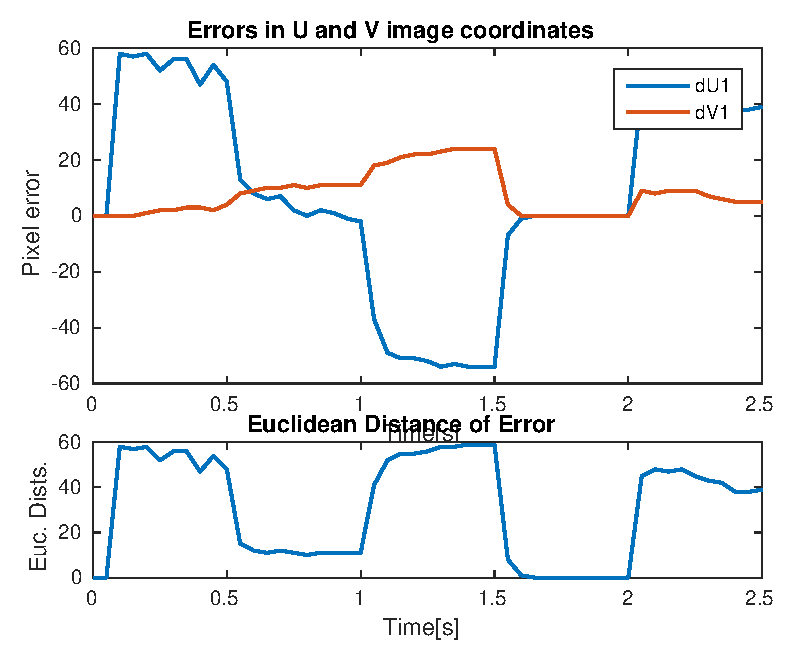
\includegraphics[width=0.49\linewidth]{fig/MediumSequence_dT50_1Pt_following_error_vs_time.eps}
	}\hfill
	\subfloat[Tracking 3 Points]
	{
		\label{fig:MediumSequence_dT50_MPt_following_error_vs_time}
		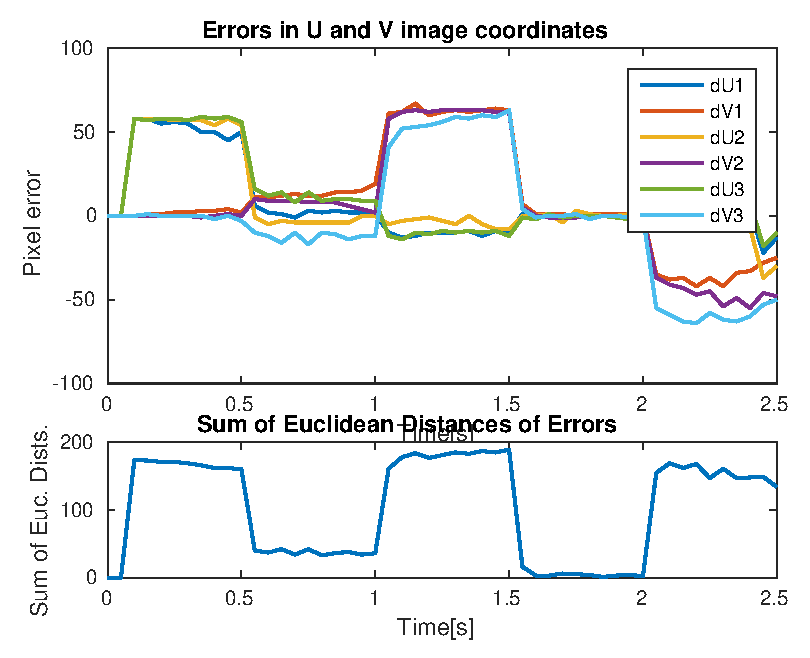
\includegraphics[width=0.49\linewidth]{fig/MediumSequence_dT50_MPt_following_error_vs_time.eps}
	}%
	\caption{Medium Sequence, \texttt{deltaT = 50} ms}
	\label{fig:MediumSequence_dT50_following_error_vs_time}
\end{figure}
\begin{figure}[!htp]
	% Maximum length
	\subfloat[Tracking Single Point]
	{
		\label{fig:MediumSequence_dT35_1Pt_following_error_vs_time}
		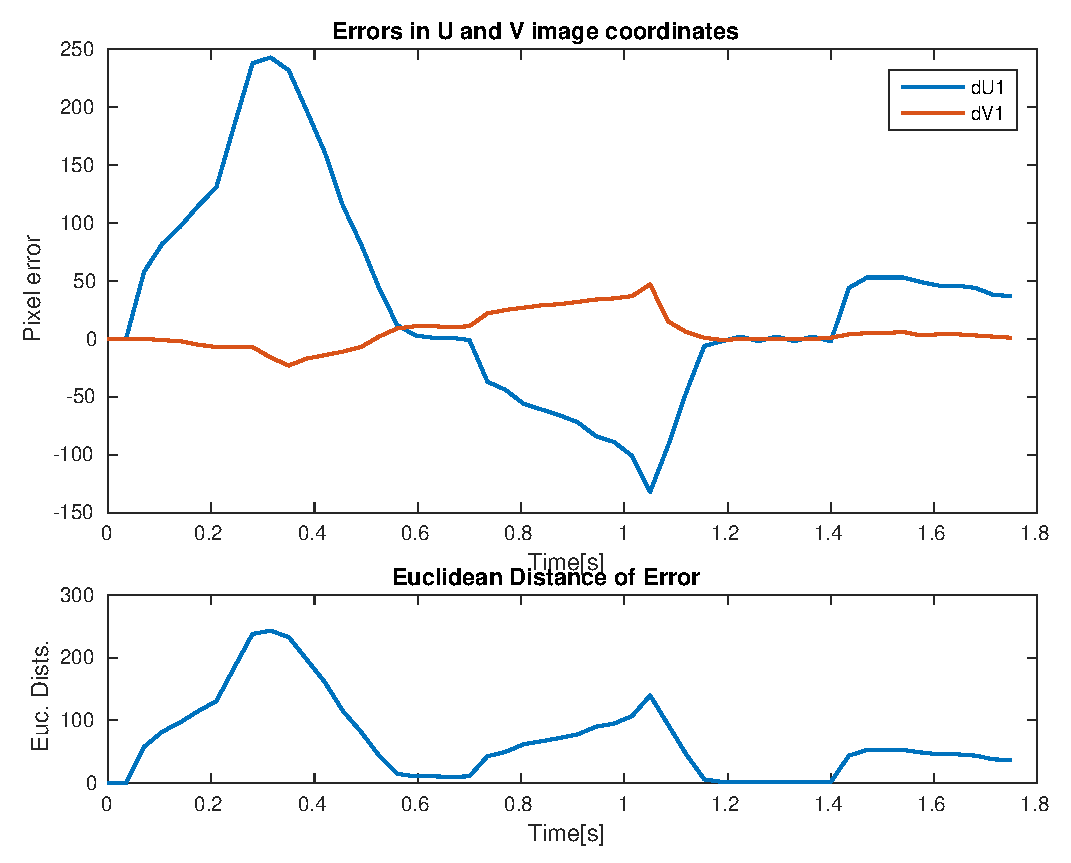
\includegraphics[width=0.49\linewidth]{fig/MediumSequence_dT35_1Pt_following_error_vs_time.eps}
	}\hfill
	\subfloat[Tracking 3 Points]
	{
		\label{fig:MediumSequence_dT35_MPt_following_error_vs_time}
		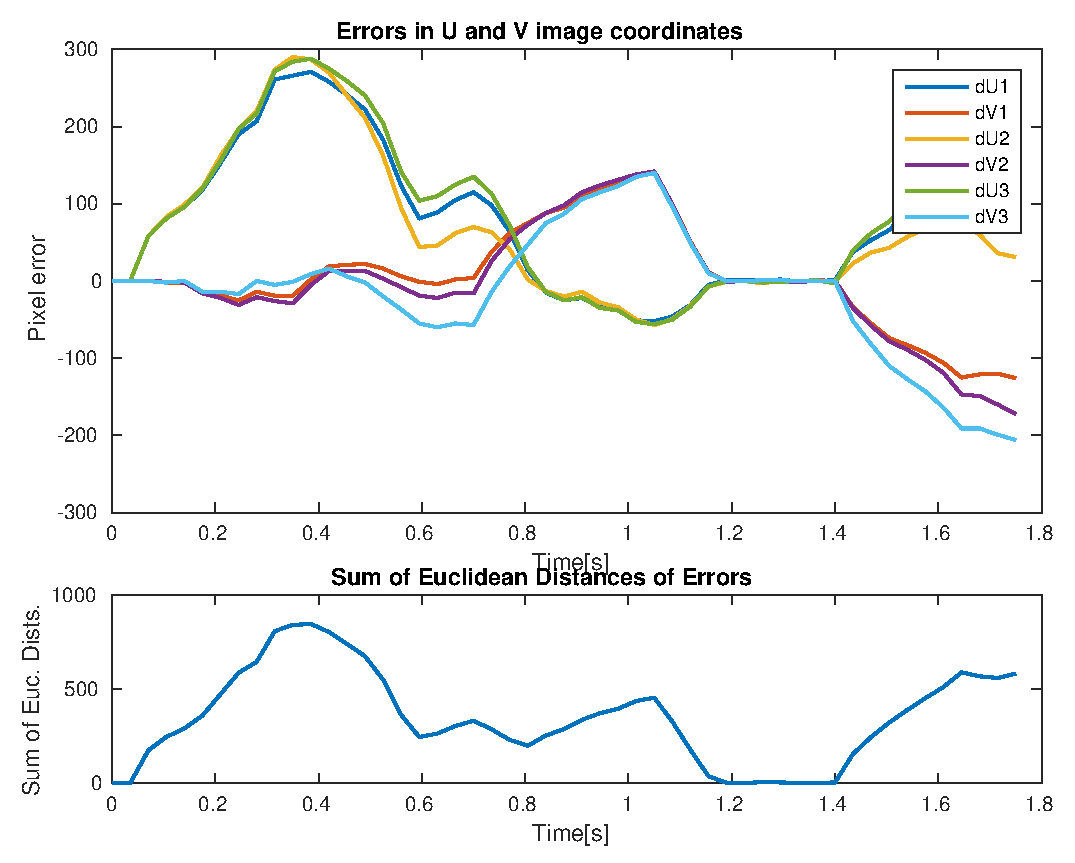
\includegraphics[width=0.49\linewidth]{fig/MediumSequence_dT35_MPt_following_error_vs_time.eps}
	}%
	\caption{Medium Sequence, \texttt{deltaT = 35} ms}
	\label{fig:MediumSequence_dT35_following_error_vs_time}
\end{figure}

%% Fast Sequence
Finally the simulations for the fast sequence are plotted on figures \ref{fig:FastSequence_dT100_following_error_vs_time} and \ref{fig:FastSequence_dT35_following_error_vs_time}.
\begin{figure}[!htp]
	% Maximum length
	\subfloat[Tracking Single Point]
	{
		\label{fig:FastSequence_dT100_1Pt_following_error_vs_time}
		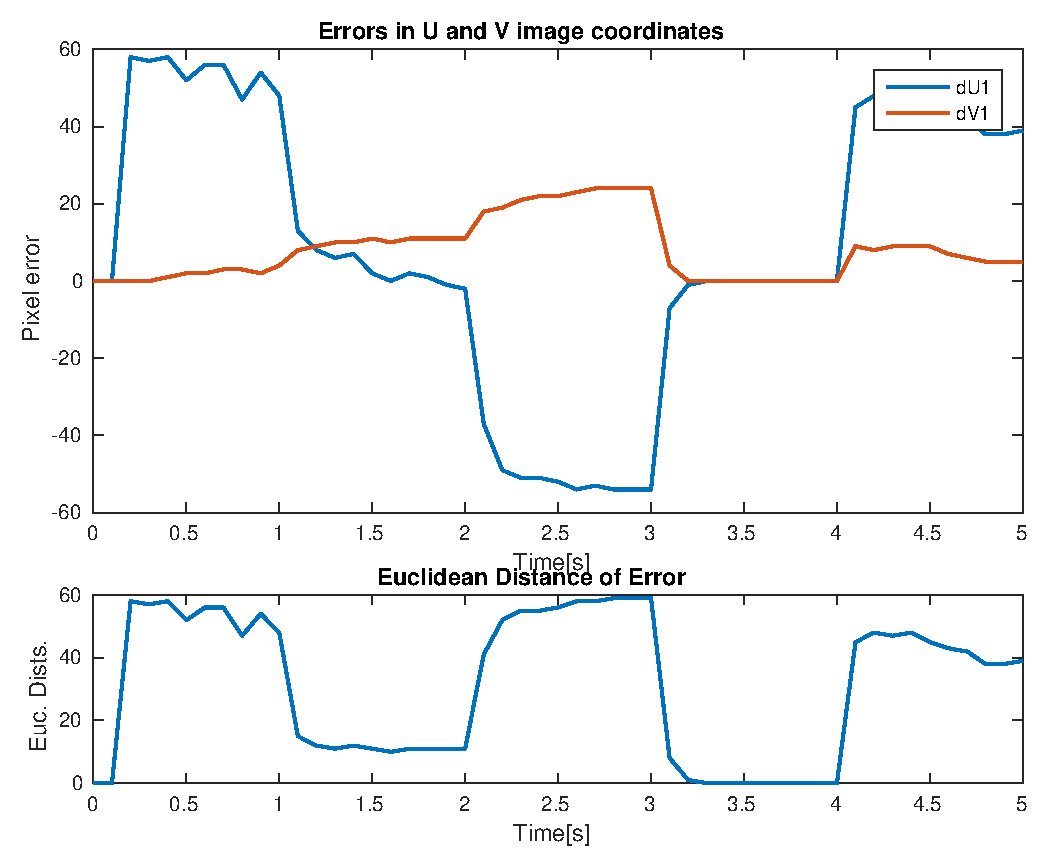
\includegraphics[width=0.49\linewidth]{fig/FastSequence_dT100_1Pt_following_error_vs_time.eps}
	}\hfill
	\subfloat[Tracking 3 Points]
	{
		\label{fig:FastSequence_dT100_MPt_following_error_vs_time}
		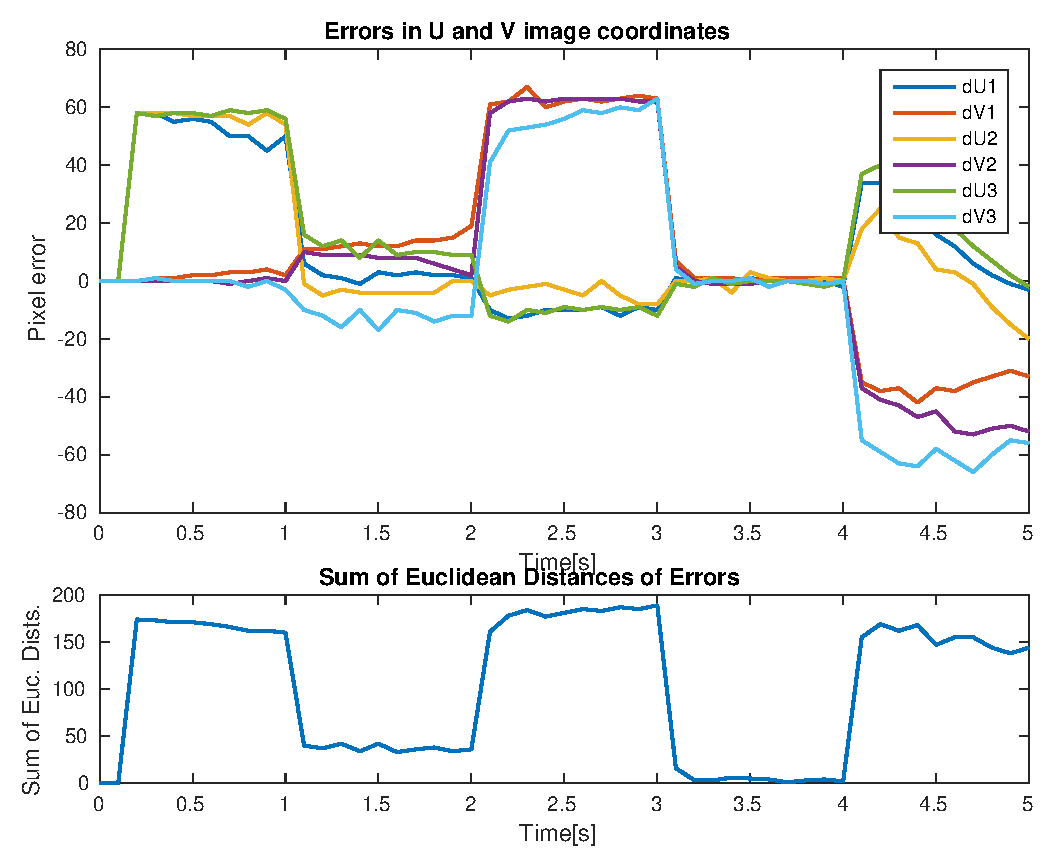
\includegraphics[width=0.49\linewidth]{fig/FastSequence_dT100_MPt_following_error_vs_time.eps}
	}%
	\caption{Fast Sequence, \texttt{deltaT = 100} ms}
	\label{fig:FastSequence_dT100_following_error_vs_time}
\end{figure}
\begin{figure}[!htp]
	% Maximum length
	\subfloat[Tracking Single Point]
	{
		\label{fig:FastSequence_dT35_1Pt_following_error_vs_time}
		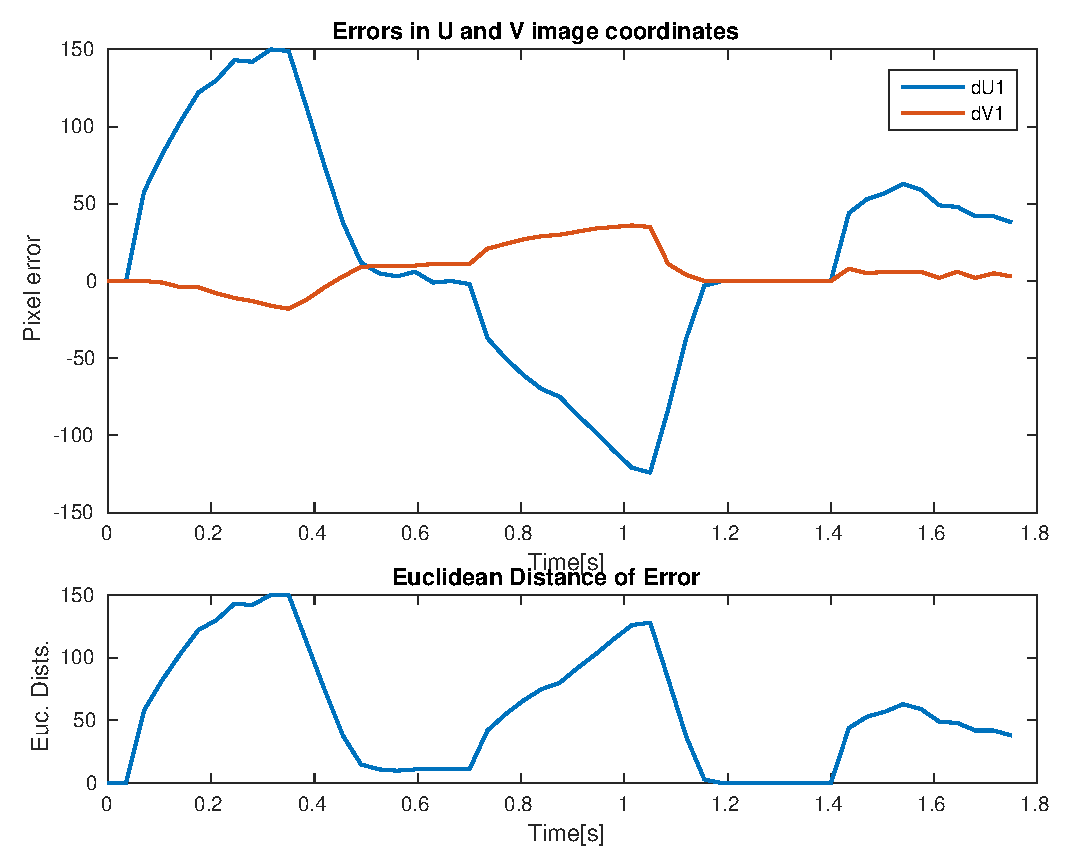
\includegraphics[width=0.49\linewidth]{fig/FastSequence_dT35_1Pt_following_error_vs_time.eps}
	}\hfill
	\subfloat[Tracking 3 Points]
	{
		\label{fig:FastSequence_dT35_MPt_following_error_vs_time}
		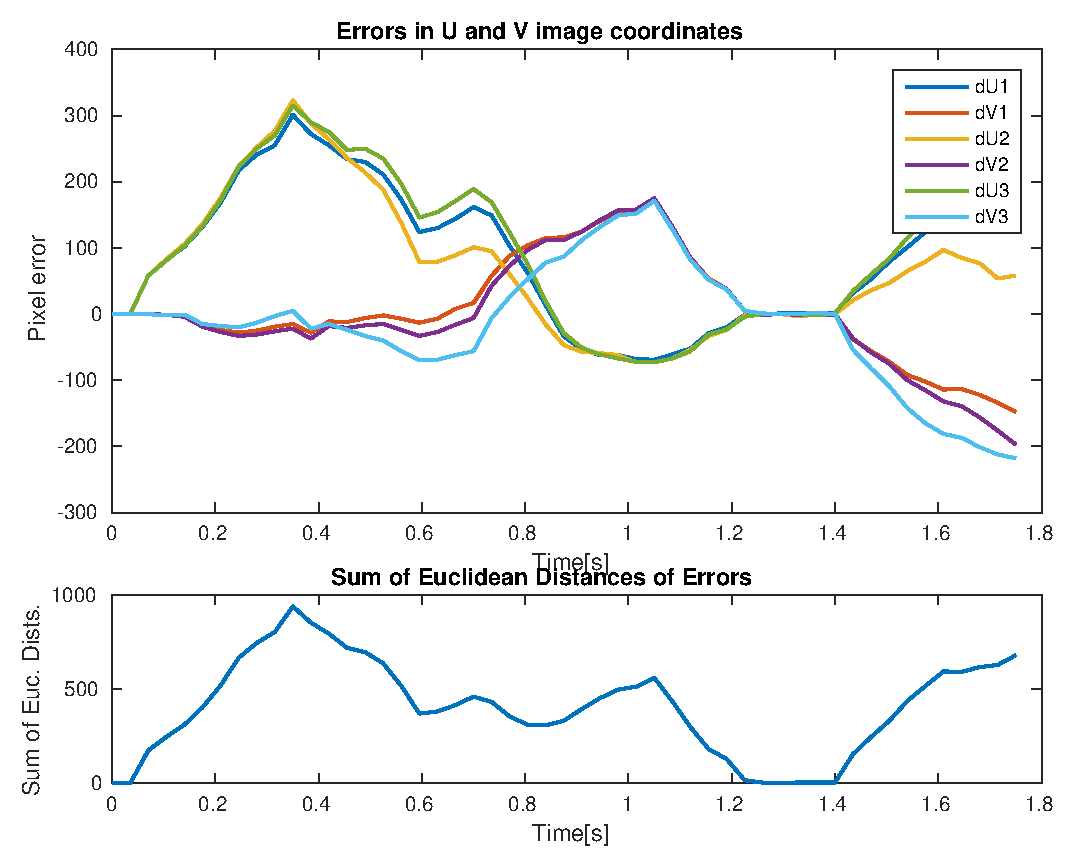
\includegraphics[width=0.49\linewidth]{fig/FastSequence_dT35_MPt_following_error_vs_time.eps}
	}%
	\caption{Fast Sequence, \texttt{deltaT = 35} ms}
	\label{fig:FastSequence_dT35_following_error_vs_time}
\end{figure}

\subsubsection*{Scaled joint positions and velocities}
Figures \ref{fig:onept} and \ref{fig:threept} show joint positions and velocities scaled to their respective limits. The data is collected from simulated visual servoing using the fast sequence with two different values of \texttt{deltaT}, 100 and 30 ms. Figure \ref{fig:onept} shows these values for single-point tracking and figure \ref{fig:threept} shows them for three-point tracking. In both figures, the left two plots show the results after setting \texttt{deltaT = 100} ms and the right two plots show runs for \texttt{deltaT = 30} ms.\par
From figure \ref{fig:onept} we see that when \texttt{deltaT = 100} ms, the robot has plenty of time to react and its joint velocities are well within limits. When \texttt{deltaT = 30} ms, the velocities come close to their limits but are mostly unsaturated. \par
From figure \ref{fig:threept} we see again that at \texttt{deltaT = 100} ms, the robot has plenty of time to react. At \texttt{deltaT = 30} ms it has little time to react and its velocities are frequently saturated. One data point has also been lost due to the fact that the feature extraction took longer than 30 ms.\par
Similar plots for the medium and slow sequences were omitted as they provided no additional insights
\begin{figure}
	\centering
	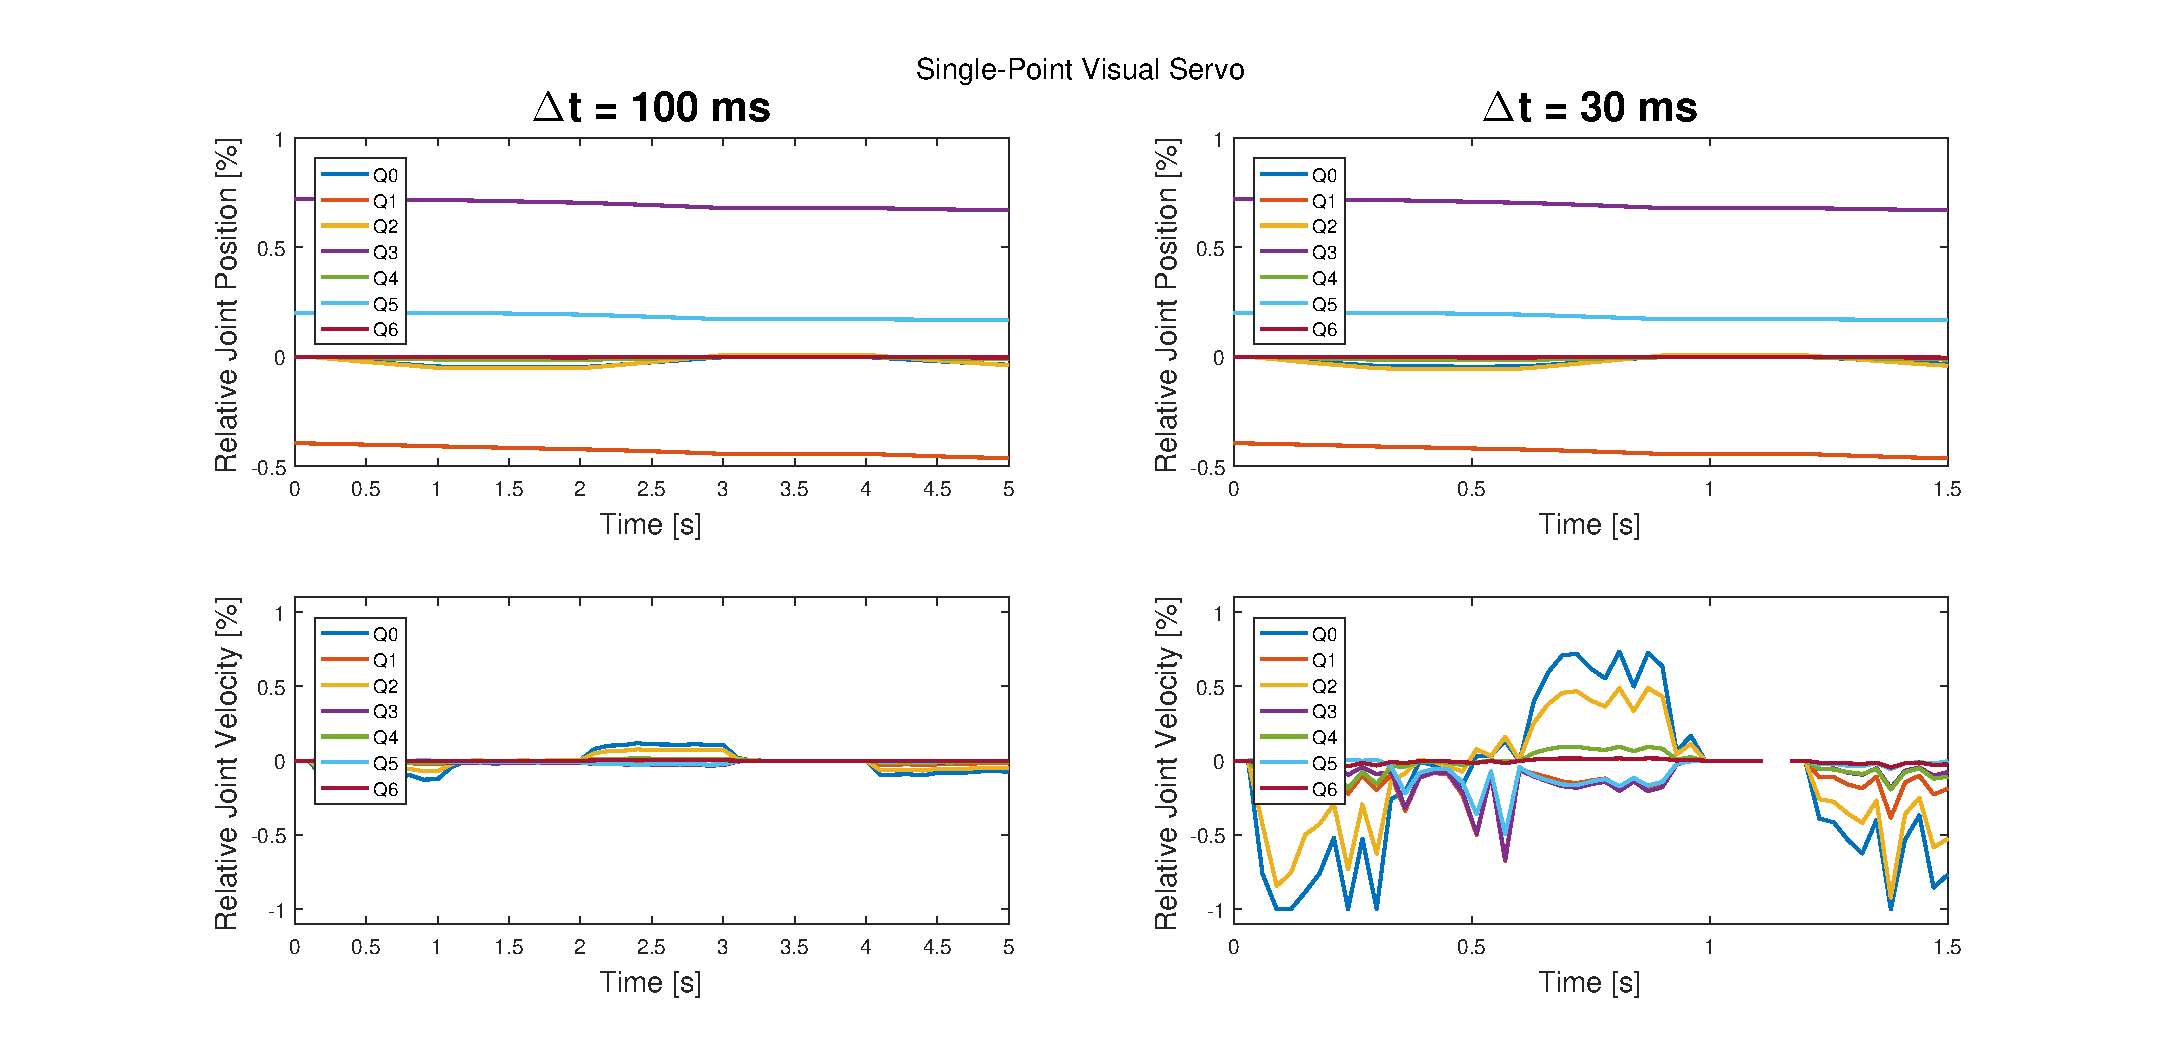
\includegraphics[width=1\linewidth, trim = 75 0 75 0]{fig/onept.eps}
	\caption{Joint positions and velocities for single-point tracking with two different \texttt{deltaT} values.}
	\label{fig:onept}
\end{figure}
\begin{figure}
	\centering
	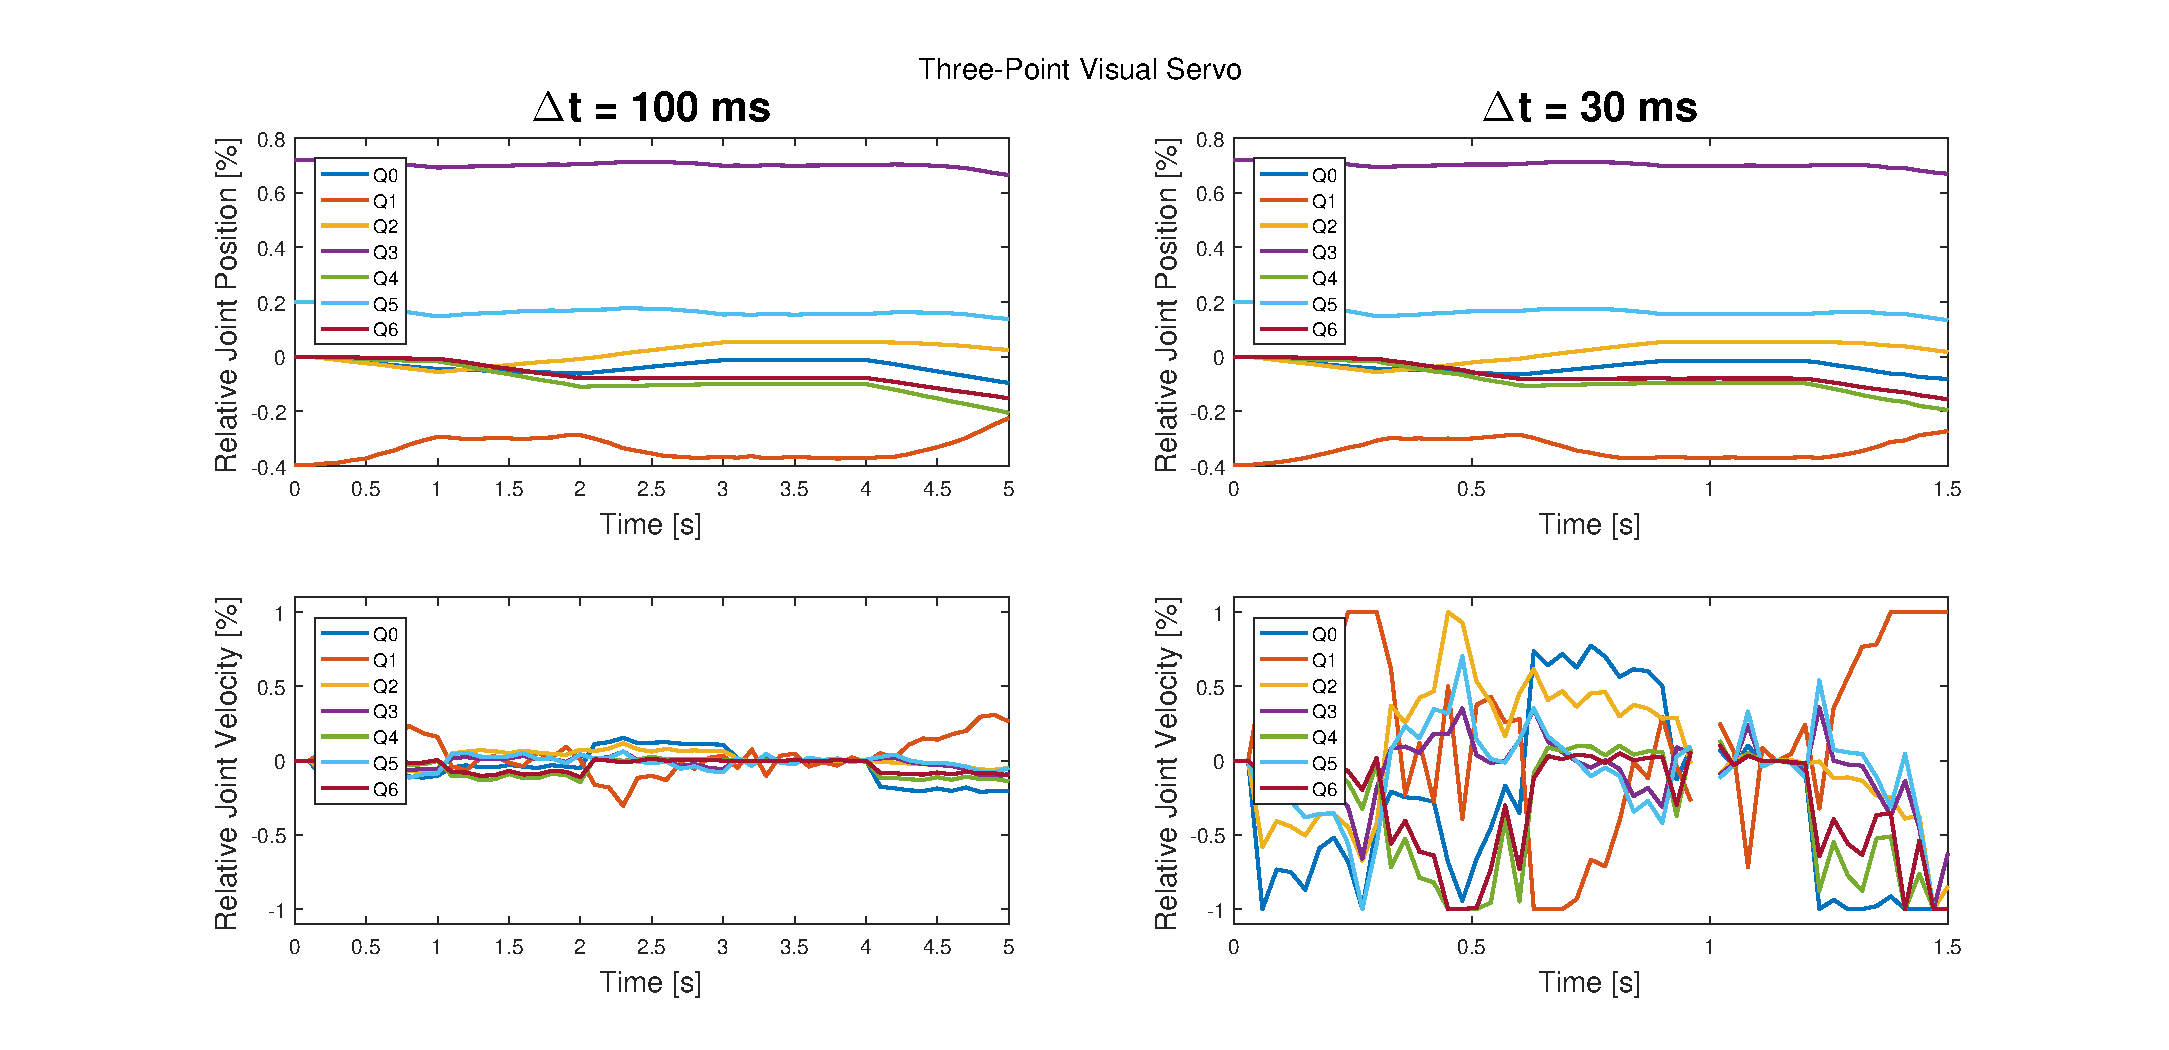
\includegraphics[width=1\linewidth, trim = 75 0 75 0]{fig/threept.eps}
	\caption{Joint positions and velocities for three-point tracking with two different \texttt{deltaT} values.}
	\label{fig:threept}
\end{figure}
\clearpage
\section{Conclusion}
For feature extraction we chose markers 1 and 2b. For marker 1 we used color segmentation and picked the three roundest blue shapes in the image. This solution was very successful and found the desired points in each image from the corresponding sequence with high accuracy.\par
For marker 2b we used hough lines and filtered out false positives by dilating and ANDing with the edges in the image. We then found the largest rectangle in the resulting image. This solution also worked for all images in the corresponding sequences but the rectangle detection was suboptimal and highly sensitive to out-of-plane rotations, resulting in a loss of precision.\par
In the robotics part we have successfully implemented visual servoing for the manipulator. By using a mathematical model for the camera and prespecified marker target points we validated the inverse kinematics computations. Even though we tried the whole sequence for the $\Delta T$ from the problem description we haven't had any problems during marker following. No adjustment of joint velocities was needed and so the maximum errors has been the same for all $\Delta T$ from the sequence. To make sure that our velocity adjustments function properly we decided to run test for even smaller values of $\Delta T$. Finally we reached a point when the marker following wasn't possible because of joint limits.\par
In the last part of the project we have successfully combined the image recognition with the visual servoing. During tests on two different computers, we have found that computation time wans't the same. This isn't really surprising, but it is an important fact to mention.  

\clearpage
\bibliographystyle{IEEEtran}
\bibliography{IEEEabrv,refs}

\end{document}
